\documentclass[a5paper,11pt]{memoir}
\usepackage[T2A,T1]{fontenc}
\usepackage[utf8]{inputenc}
\usepackage[russian]{babel}
\usepackage{multicol}
\usepackage{hyperref}
\usepackage[math]{anttor}  % set font to Antykwa Torunska
\usepackage[pages=some]{background}
\usepackage{fancyhdr}  % needed to omit chapter name on every page
\usepackage{menukeys}  % for keyboard shortcuts rendered in a special style
\usepackage[symbol]{footmisc} % for dagger footnote
\usepackage{wrapfig}
\usepackage{subcaption} % for displaying figures side by side
\usepackage{geometry}
\usepackage{fontawesome5}
\usepackage{float}

\usepackage{yfonts,color}

\usepackage{iftex} % for identifying luatex and pdftex

% my custom definitions for character avatars in dialogues
\newcommand{\secretary}{%
%\hspace{-20pt}
 
\includegraphics[height=.8\baselineskip]{images/secretary-bird-head}
}

 
\newcommand{\zebra}{%
	%\hspace{-20pt}
	
\includegraphics[height=.8\baselineskip]{images/zebra-head}
}




\ifluatex
	% we're building the special version for dyslexics, it uses a different
	% font; this can only be done with LuaLaTeX, so we wrap with an #ifdef-like
	% structure; this logic only applies when compiling with lualatex, otherwise
	% the typical pdflatex approach is taken
	
	% the font has to be copied to /usr/share/fonts/opentype/adys
	\usepackage{fontspec}
	\setmainfont{Adys}
\fi


% \usepackage{nextpage} % needed for \cleartoevenpage, to ensure the last page/cover will fold as we need

% this is to have proper quotes for Russian text <<  >> (not " ")
\usepackage{csquotes}


\newif\ifincludetranslations
\includetranslationstrue % Uncomment this line to include translations.tex




% Syntactic sugar: a command for direct speech of various characters - it will be rendered as
% a quote with an emphasis. For quoting non-speech, use \textquote
\newcommand{\say}[1]{\emph{\textquote{#1}}}


% this is used to set the metadata of the PDF itself
% see https://en.wikibooks.org/wiki/LaTeX/Hyperlinks#Customization
\hypersetup{
    pdftitle={0! Рассказы о тех, кто не заблудился},
    pdfauthor={Alex Railean},
    pdfsubject={Рассказы для детей},
    % pdfcreator={Creator},   % creator of the document
    % pdfproducer={Producer}, % producer of the document
    pdfkeywords={рассказы, образование}, % list of keywords
    pdfpagelayout=TwoPageRight, % display as 2 columns by default, useful during development and testing
}



% EXPERIMENT with this to manipulate margin size
% https://tex.stackexchange.com/a/378157/133684
% \setlrmarginsandblock{3.5cm}{2.5cm}{*}
% \setulmarginsandblock{2.5cm}{*}{1}
% \checkandfixthelayout 


\title{\begin{otherlanguage*}{russian}
0! Рассказы о тех, кто не заблудился
\end{otherlanguage*}}  
% \author{Alex Railean}
\author{}
% \date{November 2022}


% This is necessary to remove chapter titles from every page, which would be shown otherwise
% https://stackoverflow.com/a/62250429/27342
\pagestyle{fancy}
\fancyhead[R]{\thepage}
\fancyhead[L]{}
\renewcommand{\headrulewidth}{0pt}
\fancyfoot{}
%%%%%%%%%%%%%%%%%%%%%%%%%%%%%%%%%%%%%%%%%%%%



% Adjust poem titles, so they are bigger and thicker
\renewcommand{\PoemTitlefont}{%
\normalfont\huge\bfseries\centering}


% Set the right margin to 1cm and the top margin to 1.5cm.
% https://tex.stackexchange.com/a/378157/133684
\setlrmarginsandblock{*}{1cm}{1}
\setulmarginsandblock{1.5cm}{*}{1}
\checkandfixthelayout
\begin{document}
% redefine font size 14 as 14.5 using this method, because doing it at the very top of the file only lets us choose between 12 14 17...
% https://tex.stackexchange.com/questions/323443/how-to-specify-intermediate-font-sizes-in-memoir-class
% \fontsize{15pt}{14pt}\selectfont

\date{} % so no date is shown under the title
\maketitle
\begin{center}
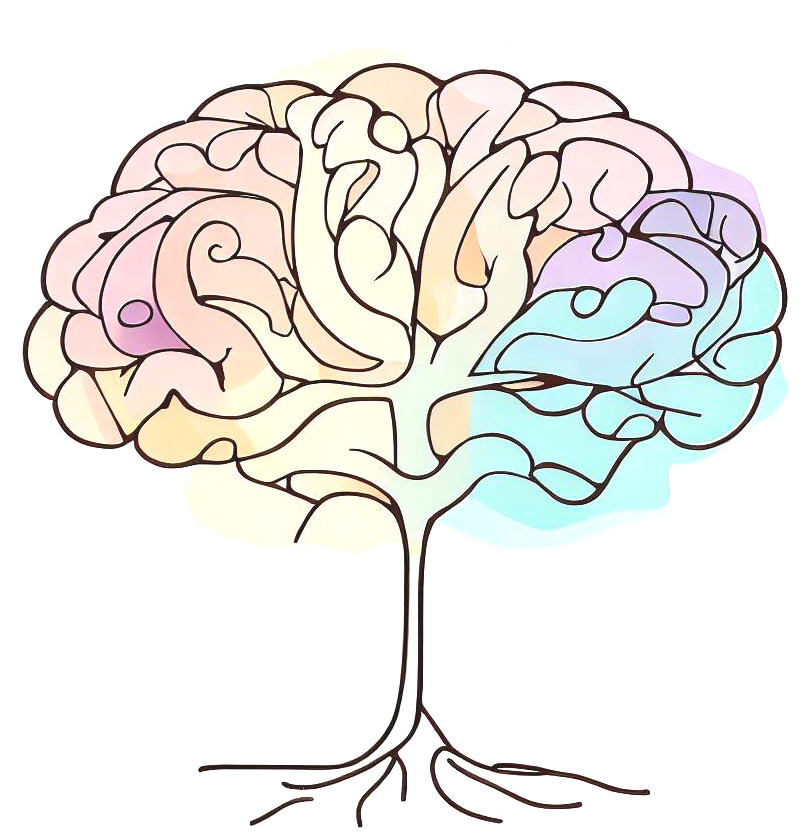
\includegraphics[height=9cm]{images/tree-cover} 

\vspace{1cm}
\tiny{
Первое издание\\
юбилейное
}


\includegraphics[width=80px]{images/laurel-3.jpeg}
\end{center}


\thispagestyle{empty}
\newpage
\thispagestyle{empty}  % to not have a page# here

\selectlanguage{russian}
% \backgroundsetup{scale=1,opacity=1,angle=0,contents={\includegraphics[width=\paperwidth,height=\paperheight]{eclipse.jpg}}}

\clearpage
% uncomment the line below to hide page number 
% \thispagestyle{empty}
\hfill

%\backgroundsetup{scale = 1, angle = 0, opacity = 0.02, contents = {\includegraphics[width = \paperwidth, height = \paperheight] {images/mountains.pdf}}}
%\BgThispage


\addto\captionsrussian{ 
}
% so the table of contents itself is not shown in the table of contents
%\begin{KeepFromToc}
 % \tableofcontents
%\end{KeepFromToc}

%\backgroundsetup{scale = 1, angle = 0, opacity = 0.9, contents = {\includegraphics[width = \paperwidth, height = \paperheight] {images/camel}}}
%\BgThispage


\thispagestyle{empty}  % hide page number
\newpage
\thispagestyle{empty}

\pagenumbering{arabic}  % so the second page begins with #1

\renewcommand{\thefigure}{\arabic{figure}}


%\chapter{asdsads}


\section*{Зебра, которая не заблудилась}
\yinipar{\color{red}O}днажды, давным давно, глубоко в африканской саванне, жила была зебра. Как-то решила она пойти в путешествие, чтобы получше познакомится со своим домом. Она черпнула немного воды из реки, почесала спинку о кору баобаба растущего вблизи, махнула хвостом, и пустилась в путь.

\begin{figure}[h]
	\hspace{-1cm}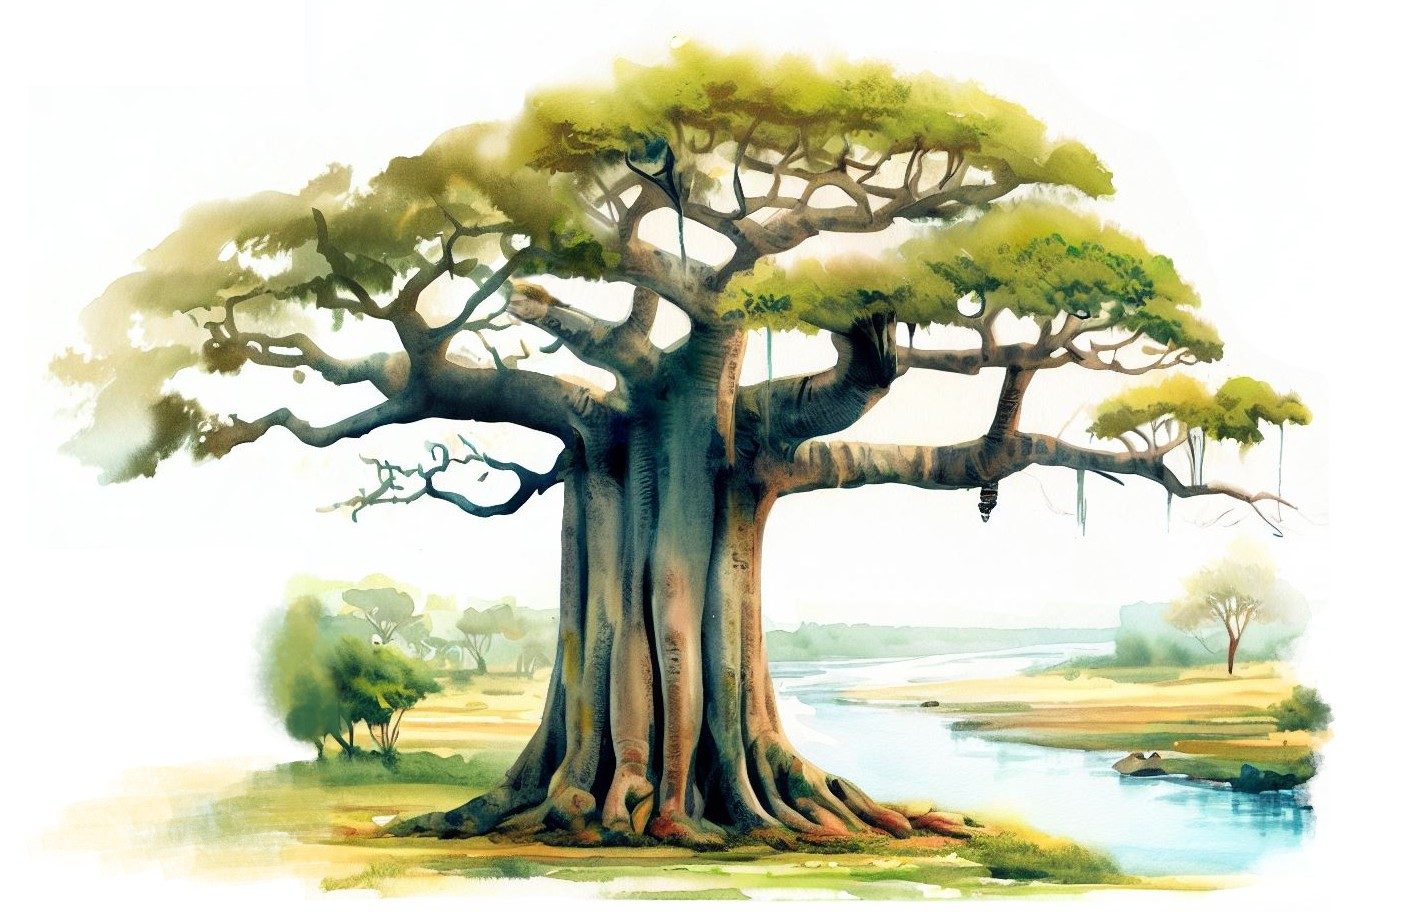
\includegraphics[width=\paperwidth]{images/baobab.jpeg}
	\caption{Баобаб (Adansonia digitata)}
\end{figure}


Она шла вдоль реки и внимательно смотрела по сторонам - таится ли в воде крокодил, нет ли хищьников в траве\ldots~\ Также, она замечала что и кто еще живет в её родных местах - кусты, деревья и форму их листьев; птицы и их формы и песни; и конечно же - на пути ей встречались носороги, слоны, буйволы и антилопы.

Зебра продолжала путешествие, не забывая часто пить водицы, особенно после длительных сегментов без тени. Когда была возможность, она кушала траву.

Шла она, шла, пока не дошла до места, где река вливается в большое озеро. Озеро было огромным -- там было много птиц, которые летали над поверхностью воды, издалека казалось что это рой пчёл, но пчёлы так не двигаются! Это было необычное зрелище! Рой летел в одну сторону, потом резко менял направление движения, потом опять резко поворачивал в другую сторону. Это повторялось без конца\ldots


\begin{figure}[H]
	\hspace{-1.02cm}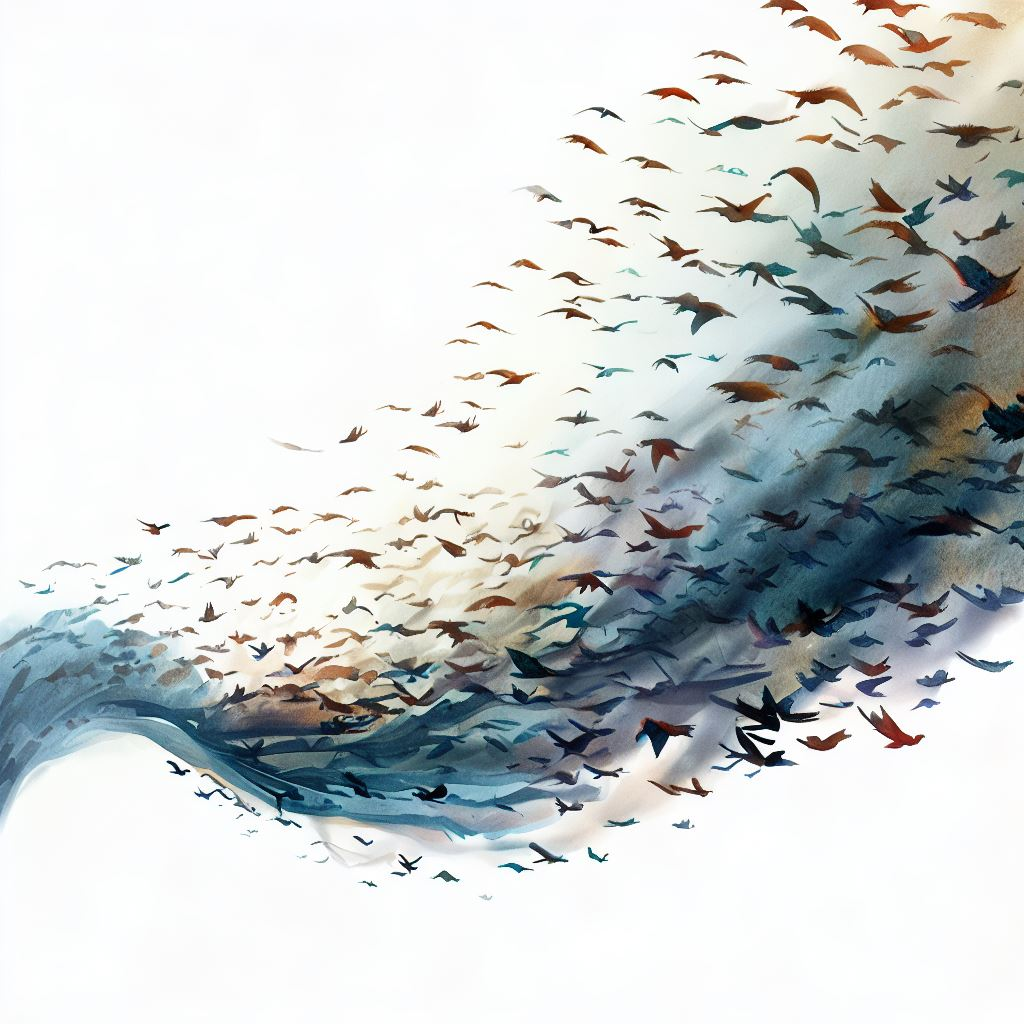
\includegraphics[keepaspectratio=false,width=\paperwidth, height=8cm]{images/bird-swarm.jpeg}
	\caption{Стая птиц}
\end{figure}


\secretary \say{Это молдавские ласточки прилетели из далекого севера. Радуются что нашли место где чувствуют себя почти как дома} -- вдруг прервал завораживающее представление голос Секретаря, который тоже наблюдал за происходящим.



Стая птиц была похоже на ленту, которая плавно перетекала из одной стороны в другую. Потом она меняла форму, передвигаясь по небу как гусеница, потом она на мгновение превращалась в одну огромную птицу, а потом распадалась на тысячи отдельных точек, потом опять превращалась в что-то другое.

\zebra \say{Север? Секретарь?}. 

\begin{figure}
	%\centering
	\vspace{-1cm}
	\hspace{-1cm}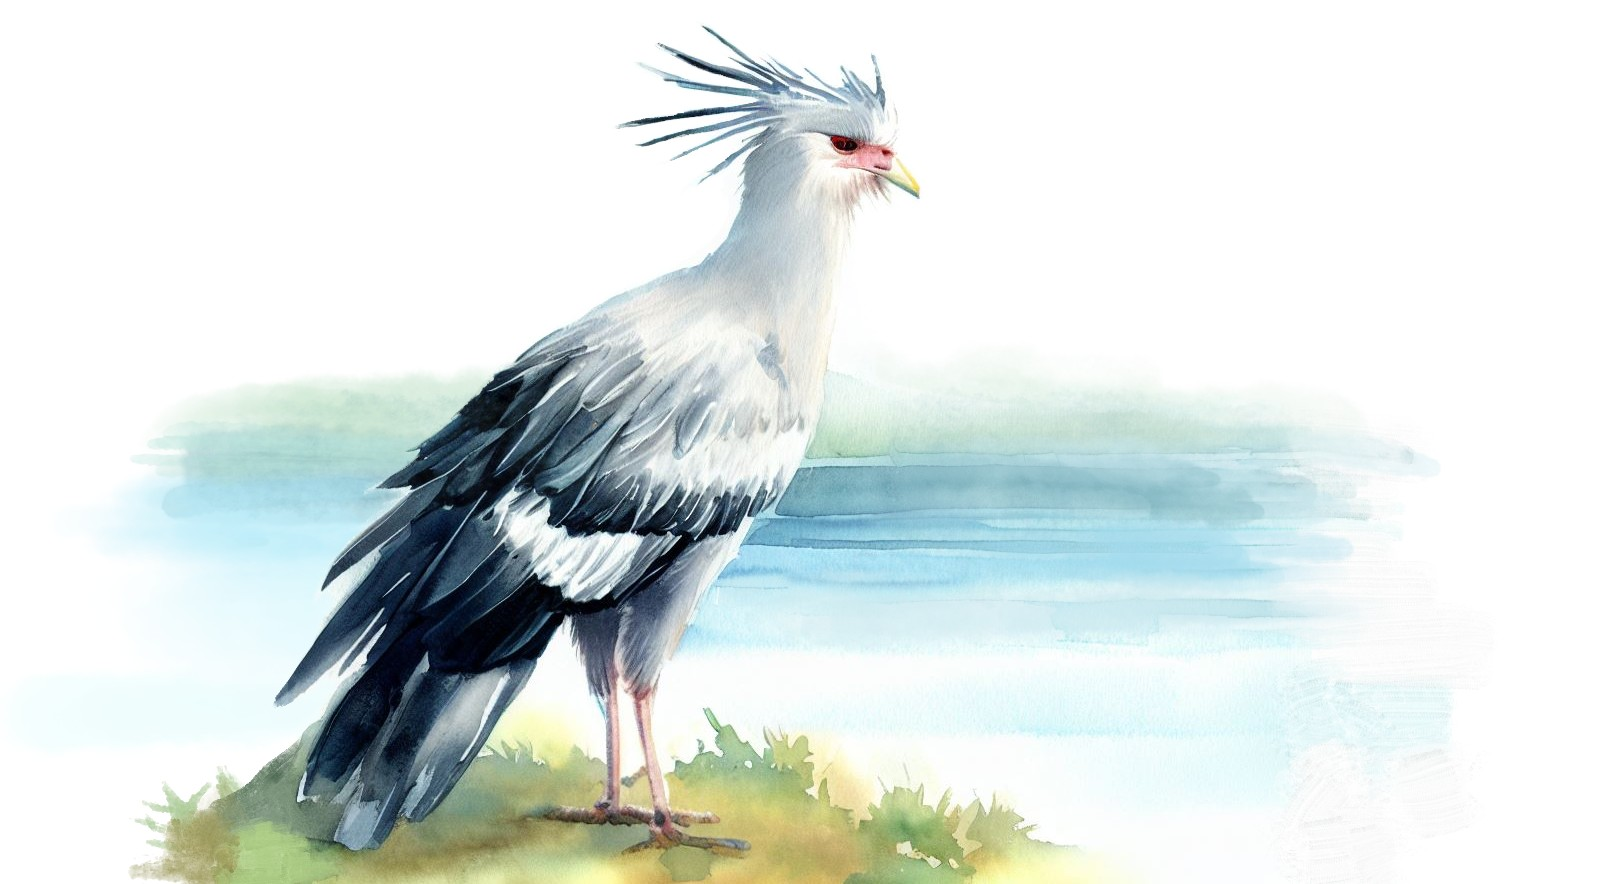
\includegraphics[width=1.2\linewidth]{images/secretary-lake.jpeg}
	\caption{Птица секретарь}
\end{figure}


\secretary \say{Да, именно так! Я птица секретарь, слежу за всем что происходит в нашей местности. Веду перепись населения, учёт ресурсов, координирую туристов, документирую потоки мигрантов, и так далее. Ты кстати, кто, что тебя сюда привело и как ты здесь оказалась?}

\zebra \say{Я зебра, пришла пешком из саванны, шла вдоль реки, пока не дошла до этого места. Сюда меня привели любопытство и зов приключений}.

\secretary \say{Аха, записал}, сказал секретарь важным голосом, хотя не было видно чтобы он что-то где-то записывал. \say{Я пишу всё в память - она у меня лучше чем у слона, поэтому меня и зовут Секретарь}, добавил на всякий случай секретарь.

\secretary \say{В округе меня называют ``Хвостуном'', потому что у меня красивый хвост}.

\zebra \say{А может Хвастуном, потому что ты хвастаешся?}, спросила зебра.

\secretary \say{Хмммм\ldots} подумал секретарь, не подавая вид что его что-то тревожит.

Они решили идти дальше вместе, так как зебра хотела узнать что еще есть за озером, да и секретарю было интересно расширить свои горизонты. Шли они, шли -- смотрели на травы, на кусты, встретились с трубкозубом, медоедом, и даже с карак\'{а}лом! % большеухой лисицей, муравьедом, they don't live there

\newgeometry{margin=0in}
\begin{figure}[t]
	\begin{subfigure}{.5\paperwidth}
		\centering
		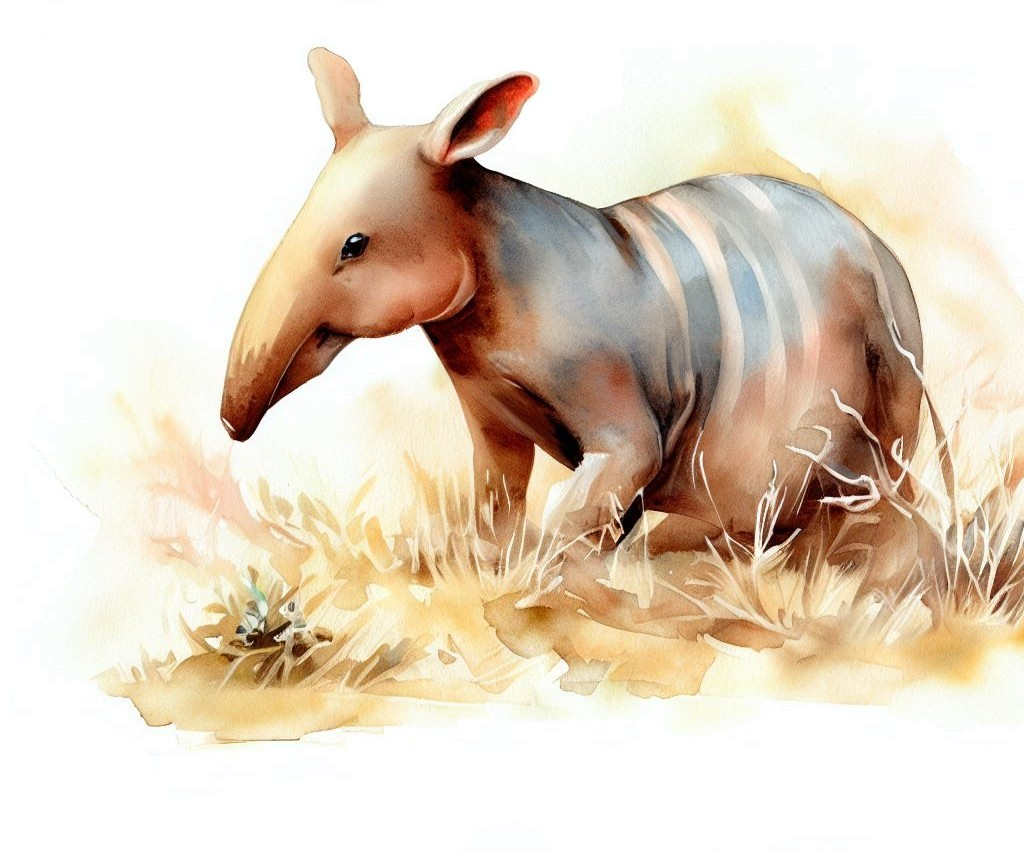
\includegraphics[width=\linewidth]{images/aardvark}
		\caption{Трубкозуб}
	\end{subfigure}%
	\begin{subfigure}{.5\paperwidth}
		\centering
		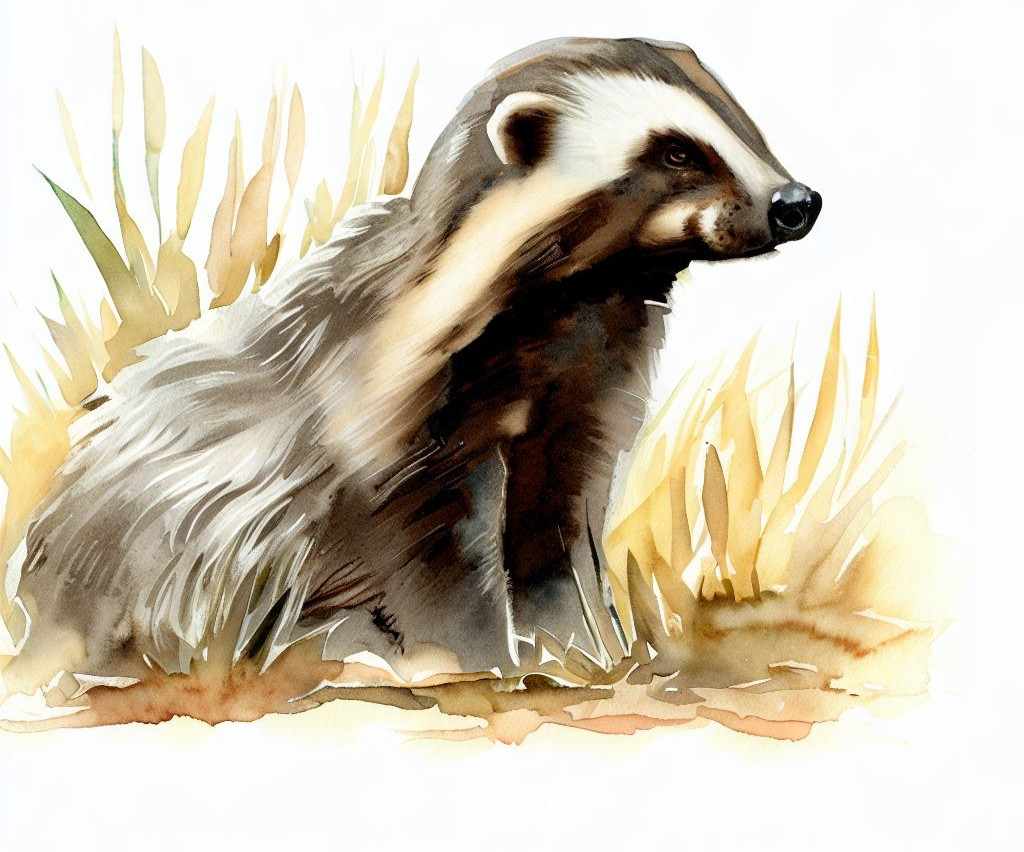
\includegraphics[width=\linewidth]{images/honey-badger}
		\caption{Медоед}
	\end{subfigure}
	
	\begin{subfigure}{.5\paperwidth}
		\centering
		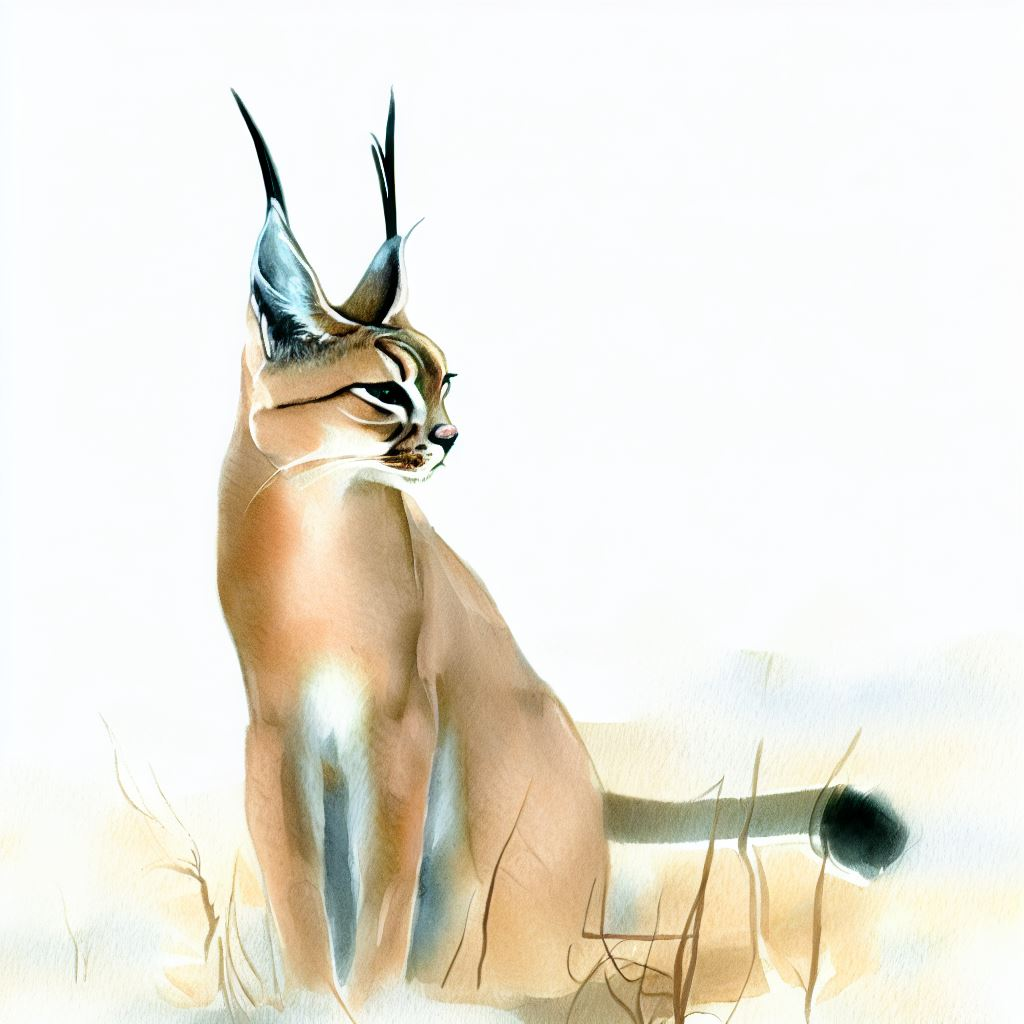
\includegraphics[width=\linewidth]{images/caracal}
		\caption{Карак\'{а}л}
	\end{subfigure}
	\begin{subfigure}{.5\paperwidth}
	\centering
	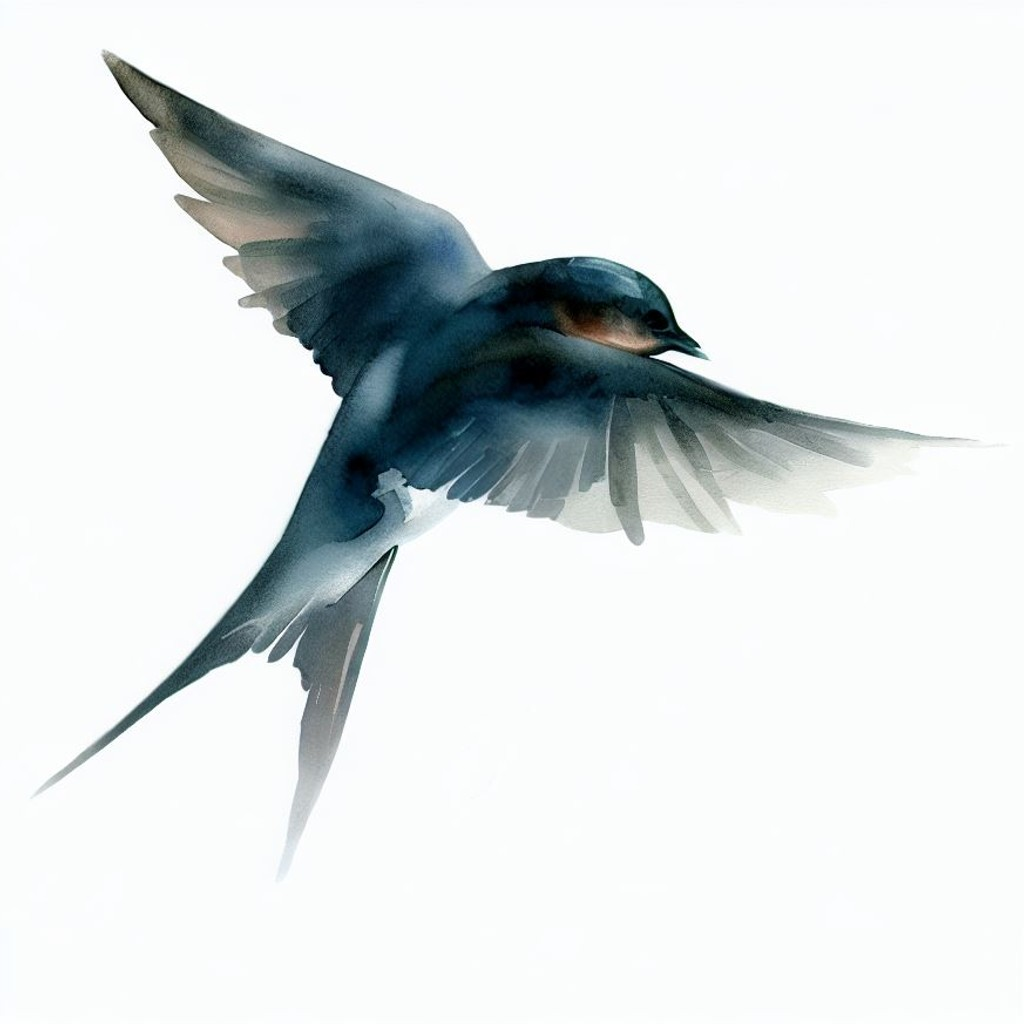
\includegraphics[width=\linewidth]{images/swallow}
	\caption{Ласточка}
\end{subfigure}
	\caption{Другие жители саванны}
\end{figure}

\restoregeometry

Время летело, и вскоре перед ними раскрылось удивительное зрелище. Небо пожелтело, потом плавно стало оранжевым, а потом и вовсе красным. Было так красиво, что никто из них не находил слов чтобы описать это. Они подождали немного, молчали вместе, хотя возможно каждый из них молчал о чём-то своём.

\begin{figure}
	\vspace{-2cm}
	\hspace{-1.02cm}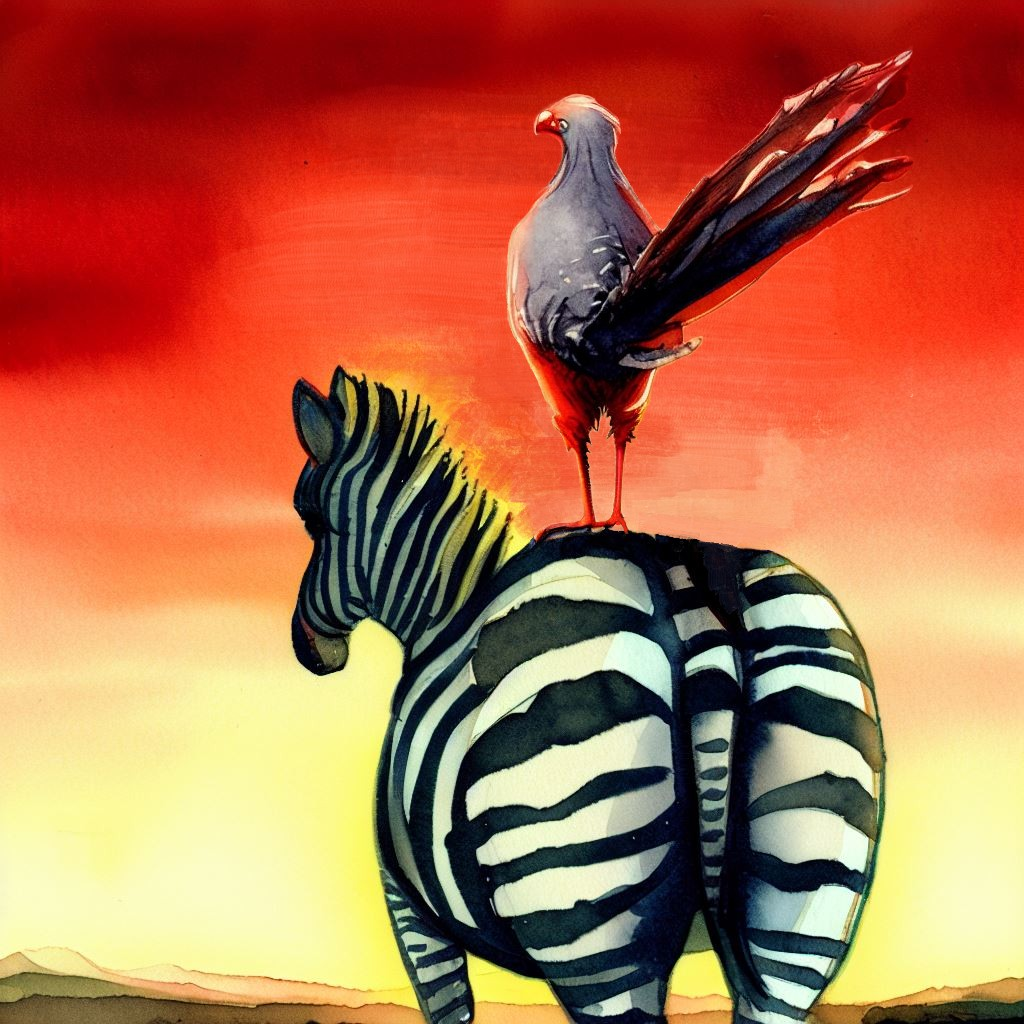
\includegraphics[width=\paperwidth]{images/rear-view-sunset-combo.jpeg}
	\caption{Начало новой дружбы}
\end{figure}


Потом они продолжили свою беседу, секретарь рассказал зебре о своих путешествиях, о далёких странах, о своём друге из Японии, об австралийской музыке, о том как он недавно ходил на хакатон, как он помог Туарегам искать соль\ldots Потом они вместе пели весёлые песни.

\secretary \say{Мы почти как бременские музыканты, только нас всего двое, и живём мы в Африке. Я однажды встретил их в поезде, когда ехал в Киль, это чуть севернее Га\ldots}, сказал незакночив мысль секретарь. Время продолжало лететь, они так хорошо разговорились, что не заметели как заблудились.
%Да, я бы с удовольствием покушала бы немного кильки.

Они оказались в неизвестном месте -- секретарь тут никогда не бывал, да и зебра о сих местах в рассказах бабушек ничего не слышала. \zebrainline \say{Не узнаю этот вид травы, листья этих кустов мне не знакомы}, подумала вслух зебра. Секретарь посмотрел по сторонам, было уже темно.

\zebra \say{Ну\ldots теперь мы влипли!} сказала зебра вздохнув.

Секретарь был с ней согласен, но пока ничего не говорил. Он думал. Зебра расстроилась, опустив голову -- \zebrainline  \say{Ох, что нам теперь делать?!}. \secretaryinline \say{Не грусти, мы подумаем и найдем решение}, сказал секретарь, хотя решения у него не было.

Печаль зебры росла, она опустила глаза, а секретарь продолжал разговаривать, предлагал идеи -- \secretaryinline \say{попробуем то\ldots{} попробуем это\ldots{}, может так\ldots{} а как насчёт этого\ldots{} может мы найдем какой-то дорожный знак, карту или другой след цивилизации?\ldots}

Зебра смотрела отчаяно на землю под ногами. \zebrainline \say{След! Точно!} воскликнула она громким голосом.

\begin{figure}[h]
	%\hspace{-1cm}
	\centering
	
\includegraphics[width=0.6\paperwidth]{images/hoofprints.jpeg}
	\caption{Следы копыт в грязи}
\end{figure}


В её голове зародился план. Она объяснила секретарю, что они могут найти обратный путь, нужно всего-навсего внимательно смотреть и находить следы. Оба обрадовались, хотя были очень усталыми.

Зебра сделала сперва один шаг, потом второй, третий, четвертый, пятый, шестой\ldots Первый шаг был самым сложным, но с каждым шагом -- уверенность росла, и зебра совсем забыла о своей усталости. Хотя была ночь, мягкий отблеск луны освещал землю достаточно хорошо.

\begin{figure}[h]
	\centering
	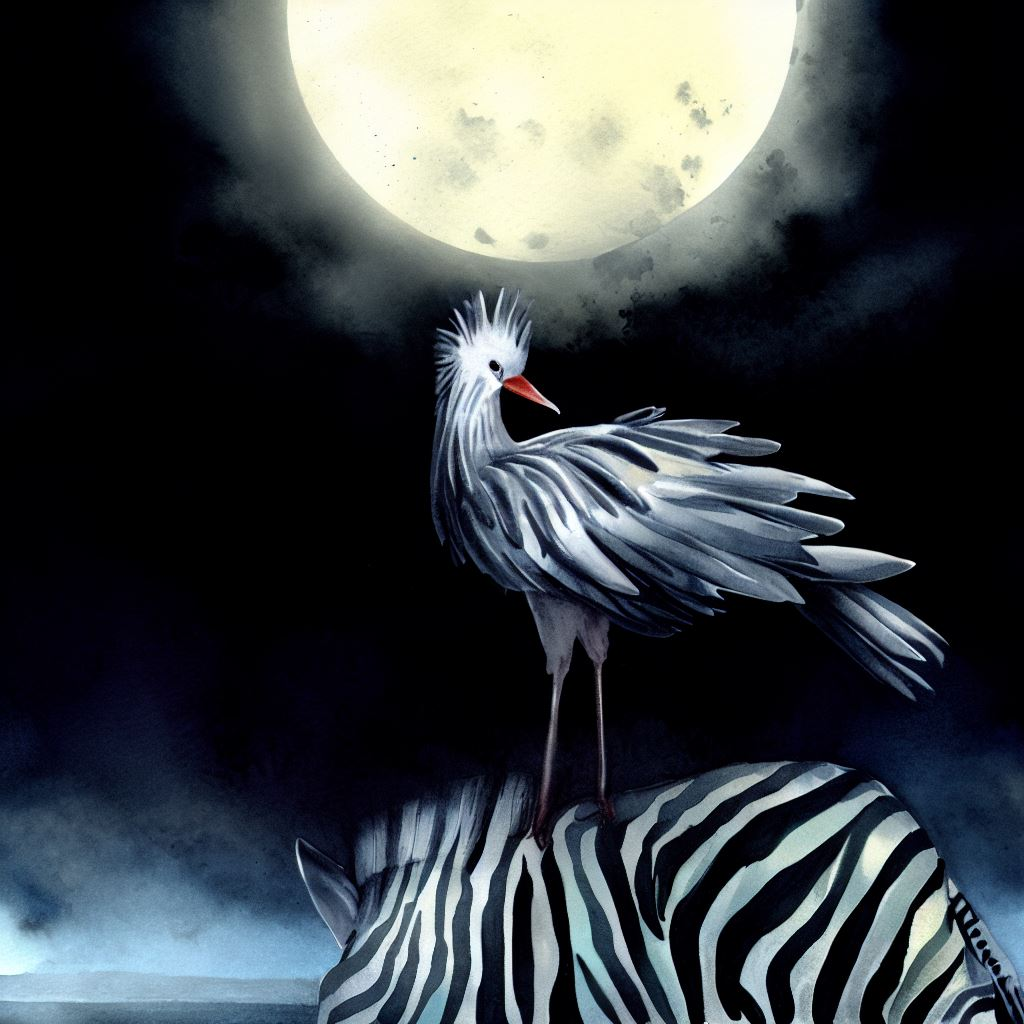
\includegraphics[width=\columnwidth]{images/moonwalk.jpeg}
	\caption{Ночное путешествие}
\end{figure}


Вскоре они вернулись к озеру, шли далее вдоль реки, встретили карак\'{а}ла, медоеда и трубкозуба\ldots Дальше и следов уже не нужно было --- эти места зебра и так знала очень хорошо.
 

Когда они дошли до баобаба, где зебра начала свой путь, было уже очень поздно и очень темно. Зебра была рада увидеть родные места. Они оба легли -- зебра под деревом, а секретарь -- на дереве.


\zebra \say{Хоть он и хвастун, но добрый, и с ним весело и интересно}, подумала зебра ложась на траву.

\secretary \say{Мы хорошо поработали в команде}, подумал в ответ секретарь.

\secretary \say{Кем мы будем? Компаньонами? Напарниками?}, спросил секретарь.

\zebra \say{Давай ``Искателями приключений''}, зевая ответила зебра.

Они мгновенно уснули.

\begin{figure}[h]
	%\centering
	\hspace{-1cm}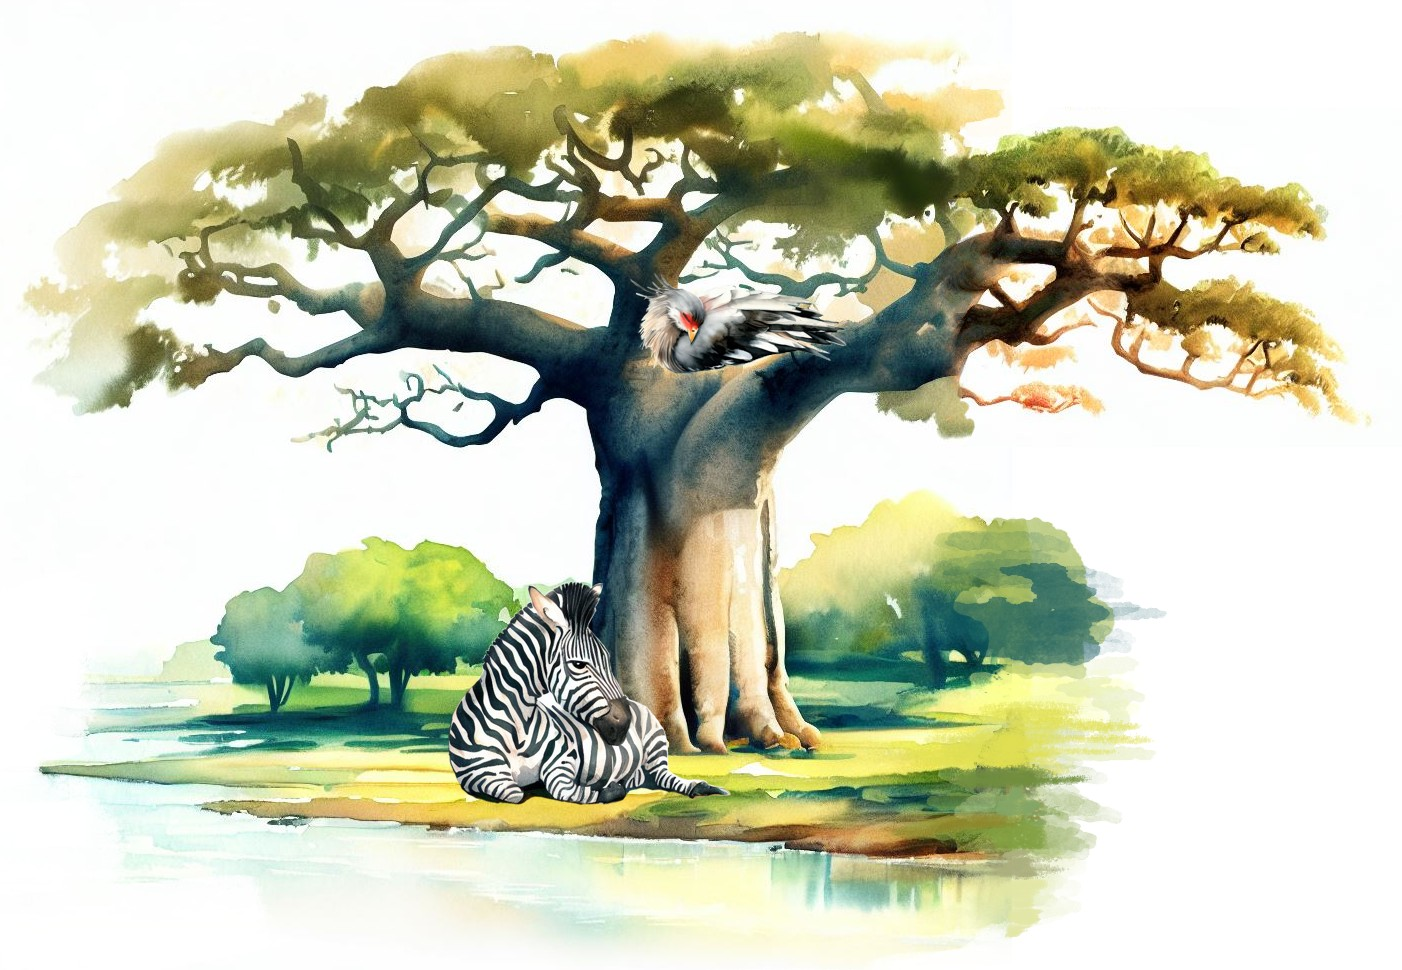
\includegraphics[width=\paperwidth]{images/baobab-nap.jpeg}
	\caption{Долгожданный отдых}
\end{figure}


\clearpage

\section*{Что растёт рядом с твоим домом}
\begin{table}[h]
	\begin{tabular}{ccc}
		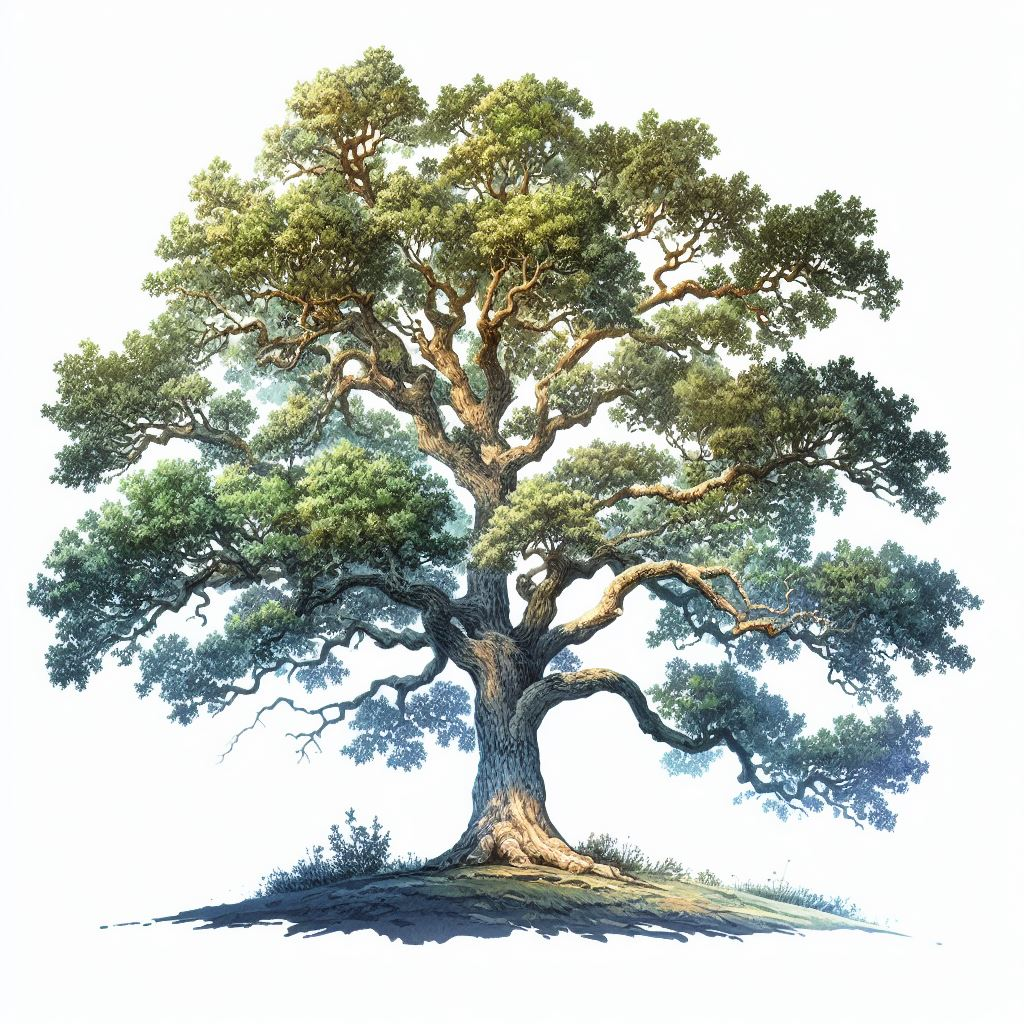
\includegraphics[height=4cm]{images/tree-guide/oak-tree} & 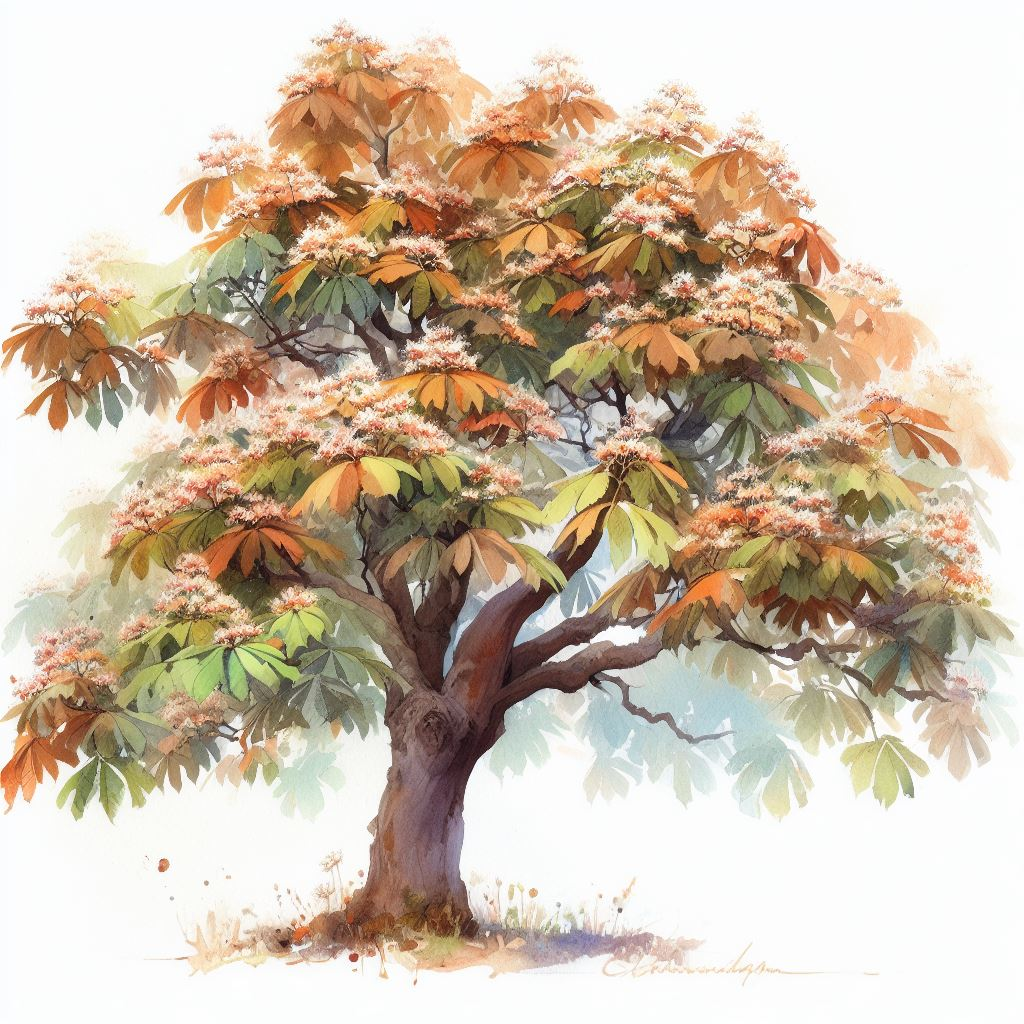
\includegraphics[height=4cm]{images/tree-guide/chestnut-tree} & 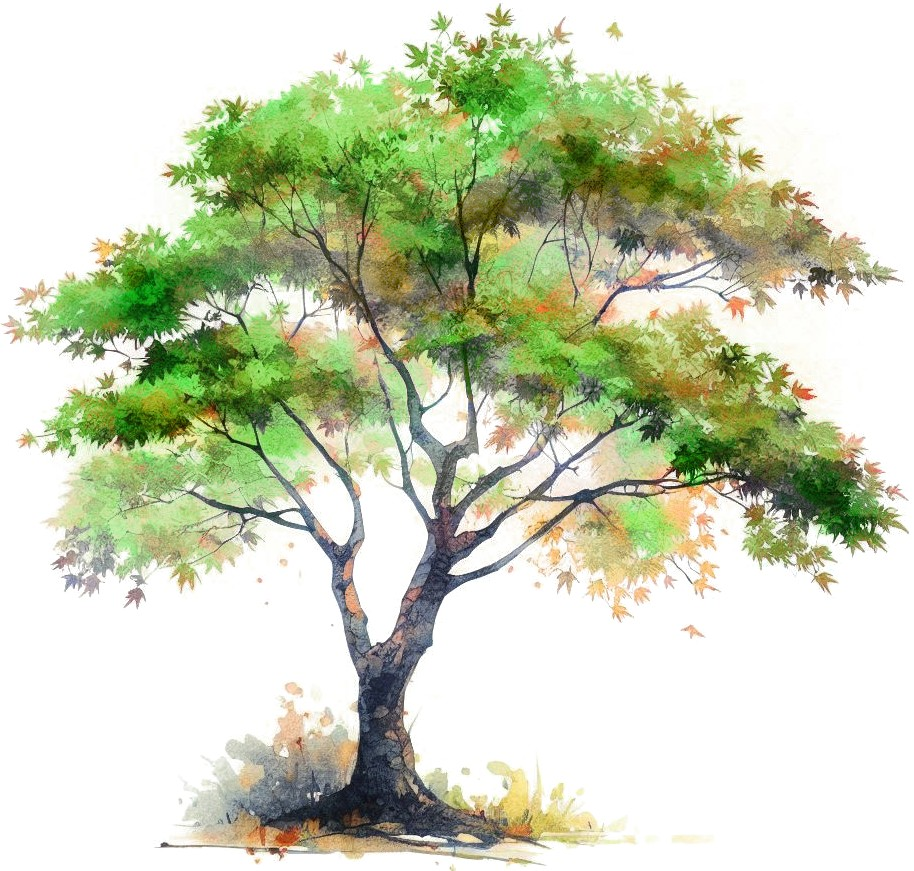
\includegraphics[height=4cm]{images/tree-guide/maple-tree}             \\
		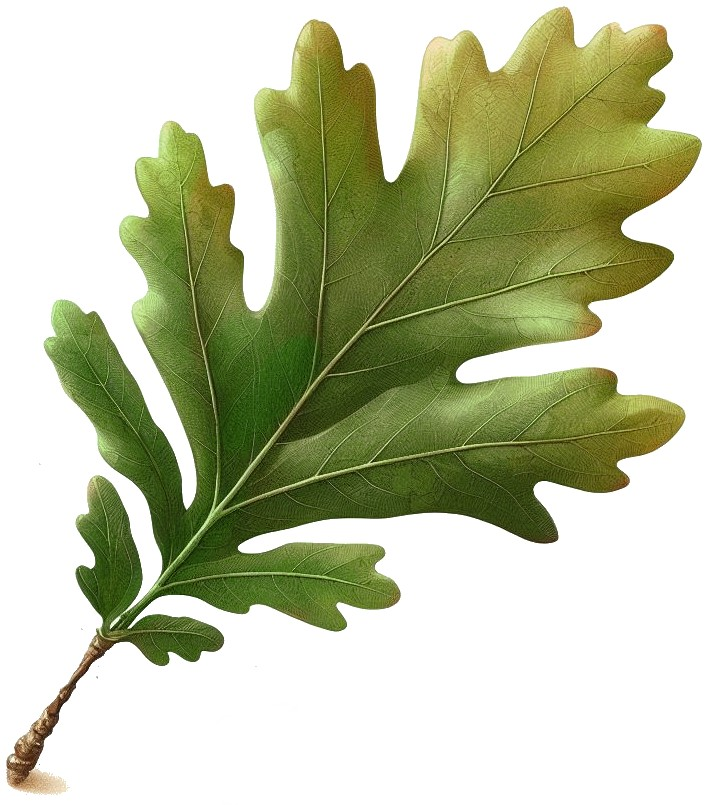
\includegraphics[height=4cm]{images/tree-guide/oak-leaf} & 
\includegraphics[height=4cm]{images/tree-guide/chestnut-leaf} & 
\includegraphics[height=4cm]{images/tree-guide/maple-leaf} \\		

		Дуб  &  Каштан        &   Клён            \\
		Stejar  &  Castan        &   Arțar            \\
		Oak  &   Horse chestnut        &   Maple, Acer \\
		die Eiche  &   die Rosskastanie     &   der Ahorn \\
		%blank line as spacing between rows
		%& & \\		
		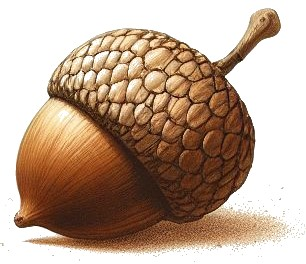
\includegraphics[height=3.4cm]{images/tree-guide/oak-acorn} & 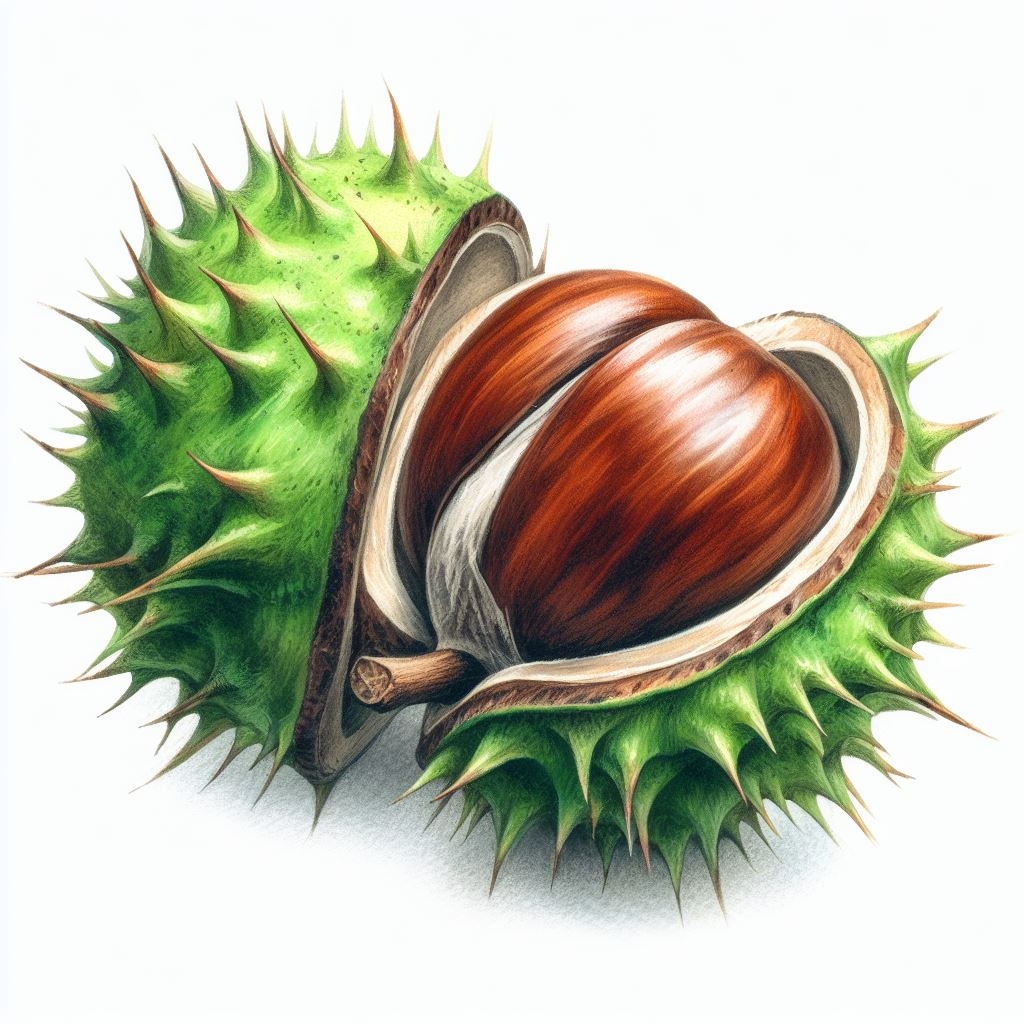
\includegraphics[height=4cm]{images/tree-guide/chestnut-fruit} &
		 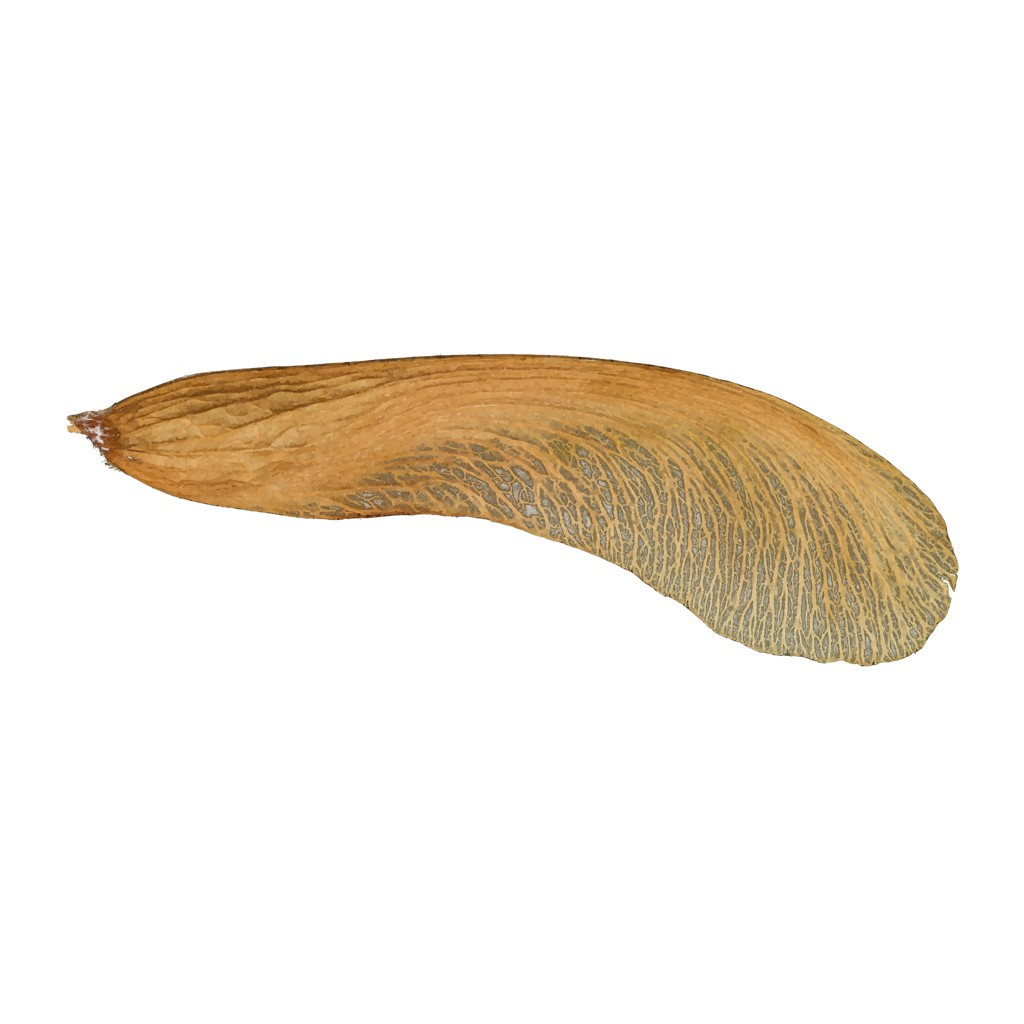
\includegraphics[height=4cm]{images/tree-guide/maple-samara} \\
		Жёлудь       &  Каштан    &     Крылатка  \\    
		Ghindă       &  Castan    &     Samară  \\    
		Acorn        &  Conker	  & Samara  \\    
		die Eichel &  die Kastanie    &     die Flügelnuss\\    
	\end{tabular}
\end{table}

\clearpage
\begin{table}[h]
	\begin{tabular}{ccc}
		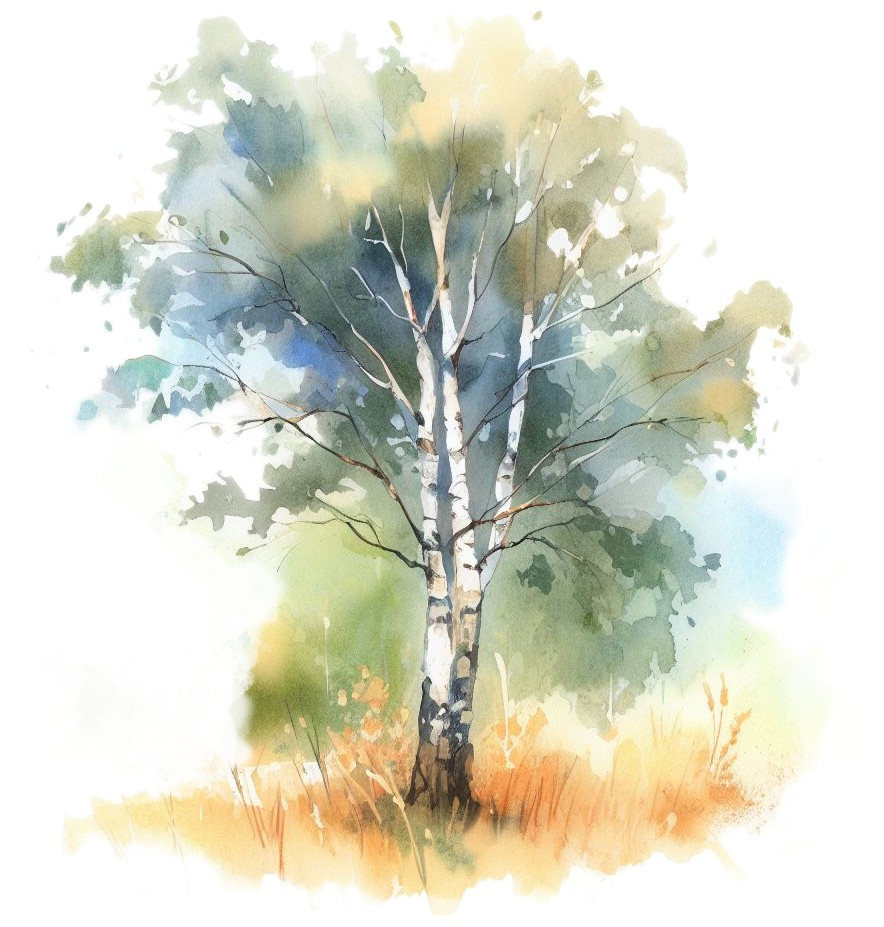
\includegraphics[height=4cm]{images/tree-guide/birch-tree} & 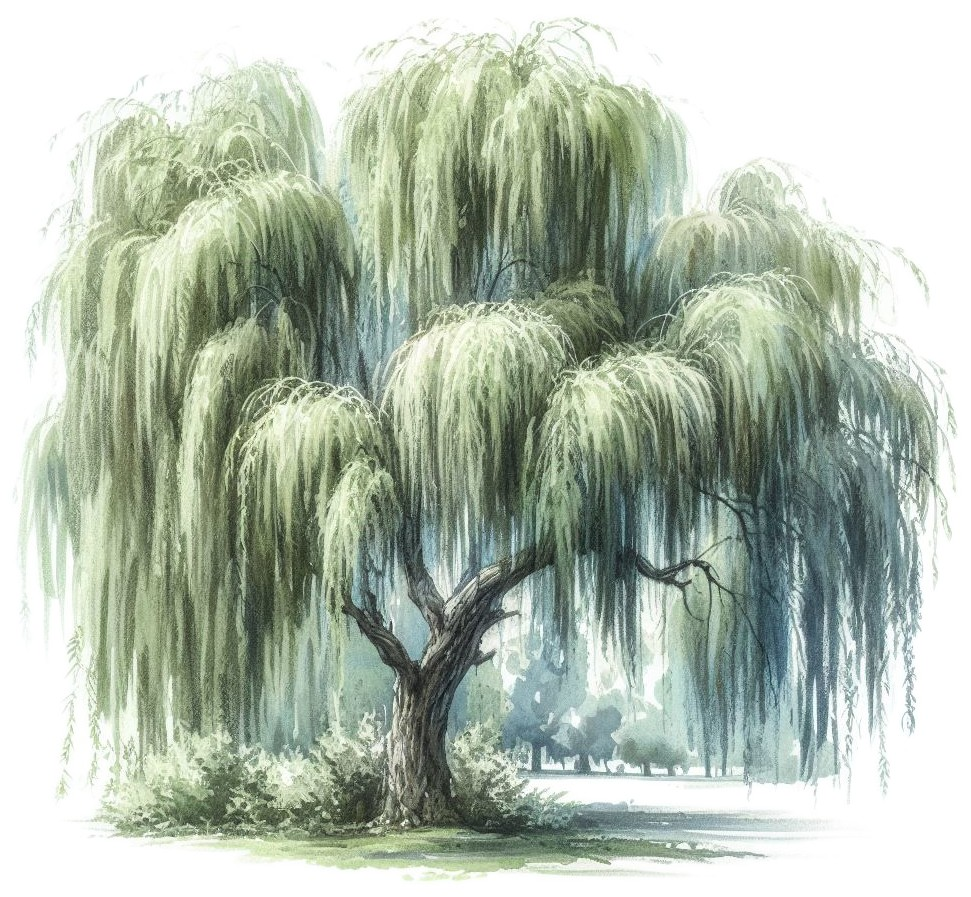
\includegraphics[height=4cm]{images/tree-guide/willow-tree} & 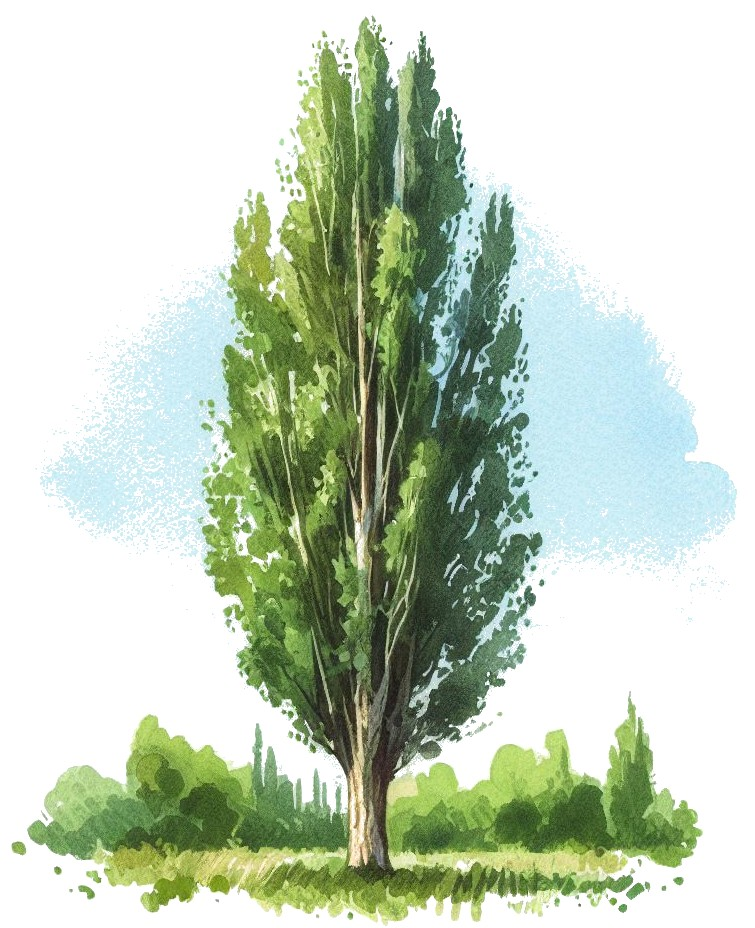
\includegraphics[height=4cm]{images/tree-guide/populus-tree}             \\
		%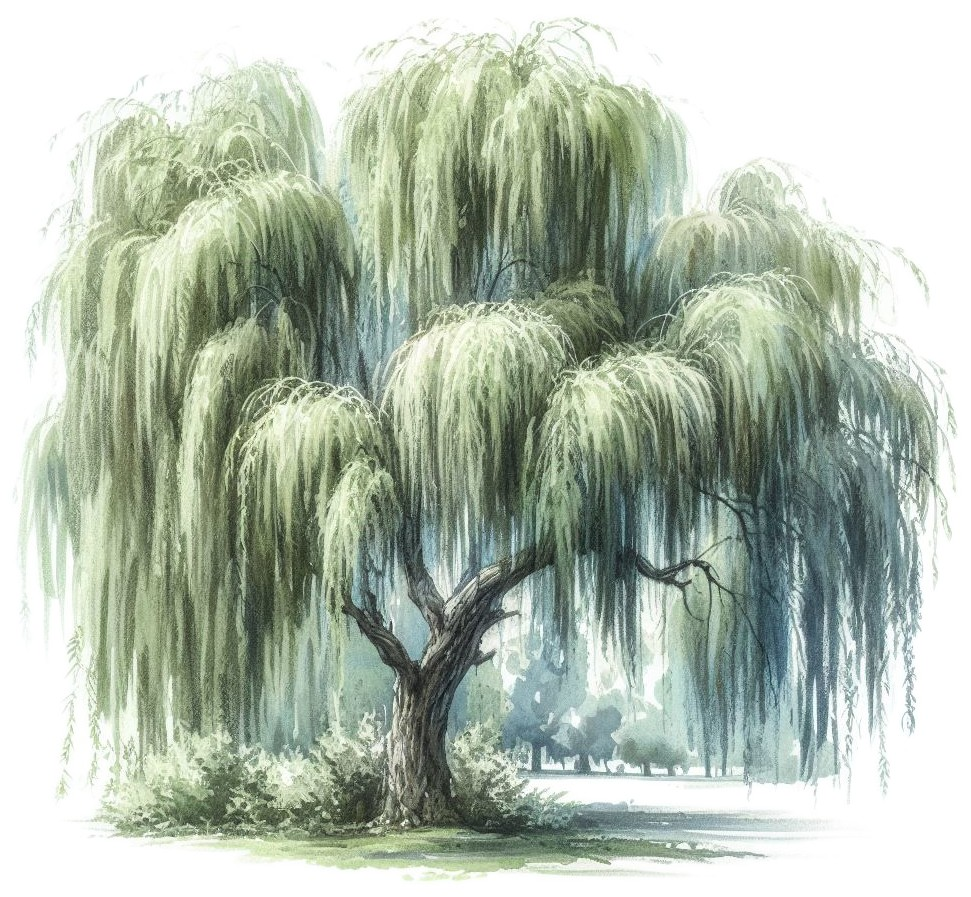
\includegraphics[height=4cm]{images/tree-guide/willow-tree} & 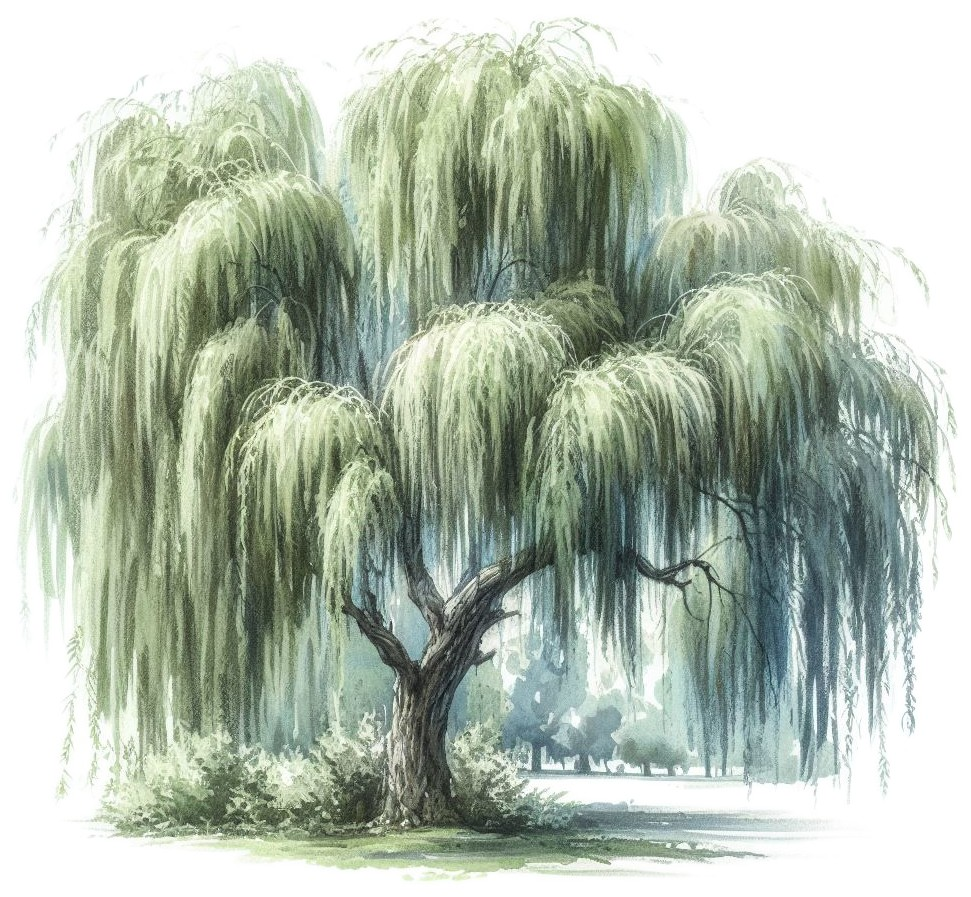
\includegraphics[height=4cm]{images/tree-guide/willow-tree} & 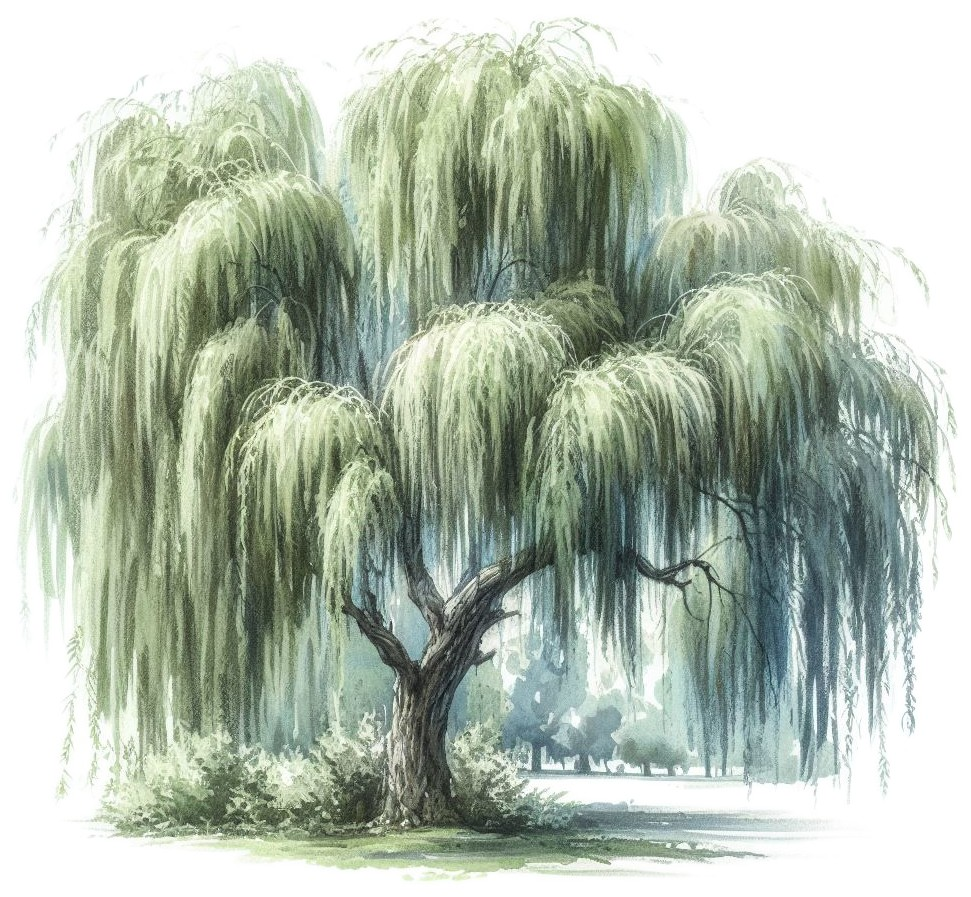
\includegraphics[height=4cm]{images/tree-guide/willow-tree} \\		
		
		Берёза  &  Ива        &   Тополь            \\
		Mesteacăn  &  Salcie        &   Plop \\
		Birch  &   Weeping willow        &   Poplar \\
		die Birke  &   die Trauerweide     &   die Pappel \\
		%blank line as spacing between rows
		& & \\		
		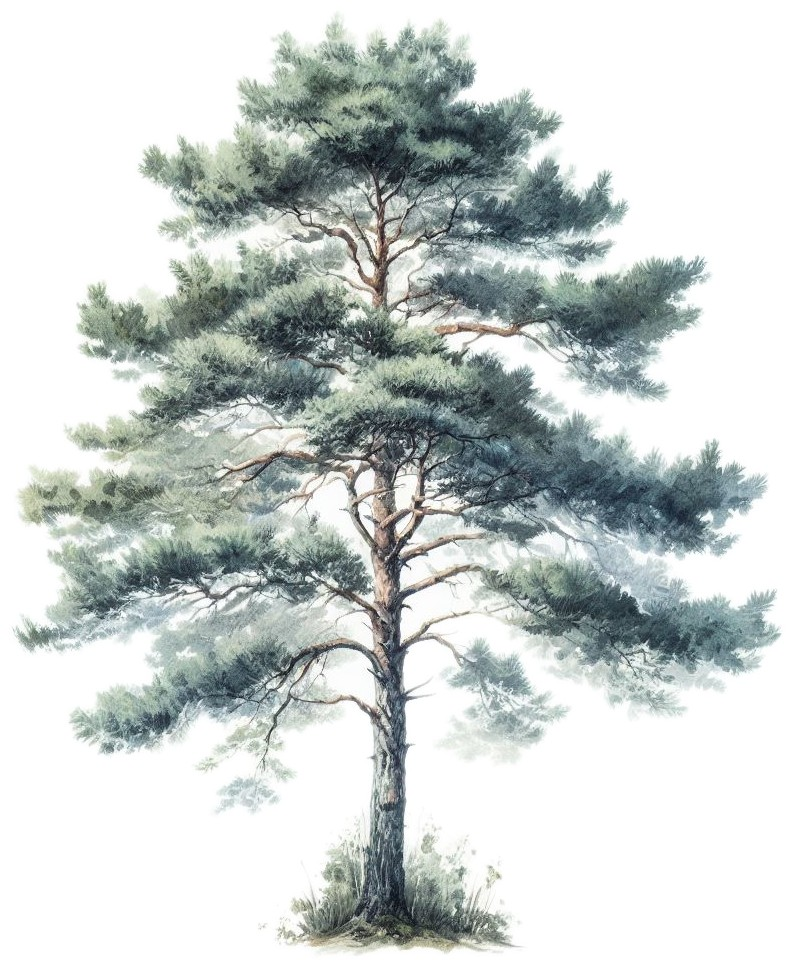
\includegraphics[height=4cm]{images/tree-guide/pine-tree} & 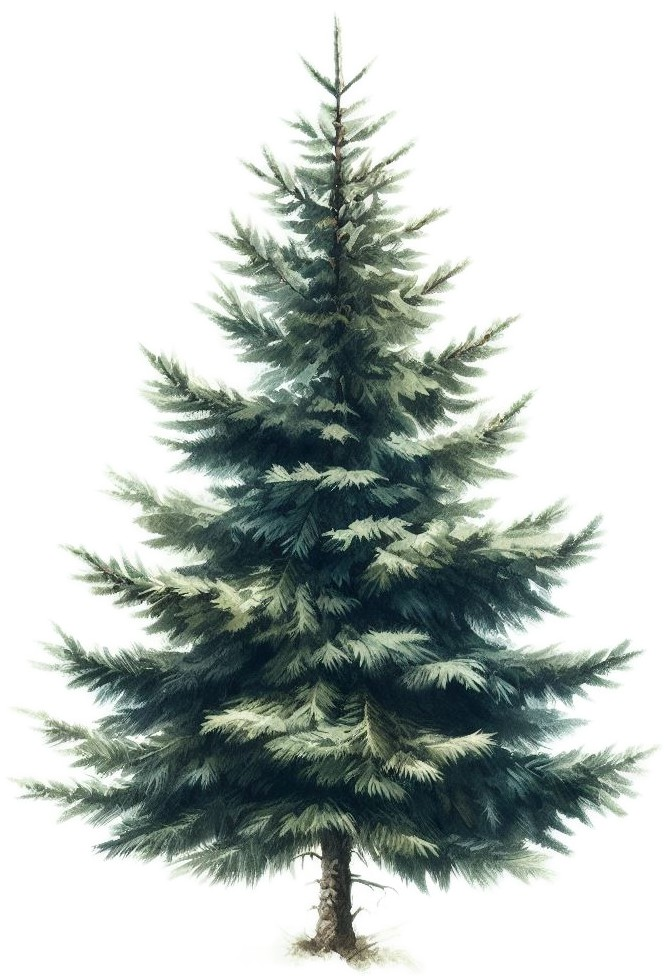
\includegraphics[height=4cm]{images/tree-guide/spruce-tree} &
		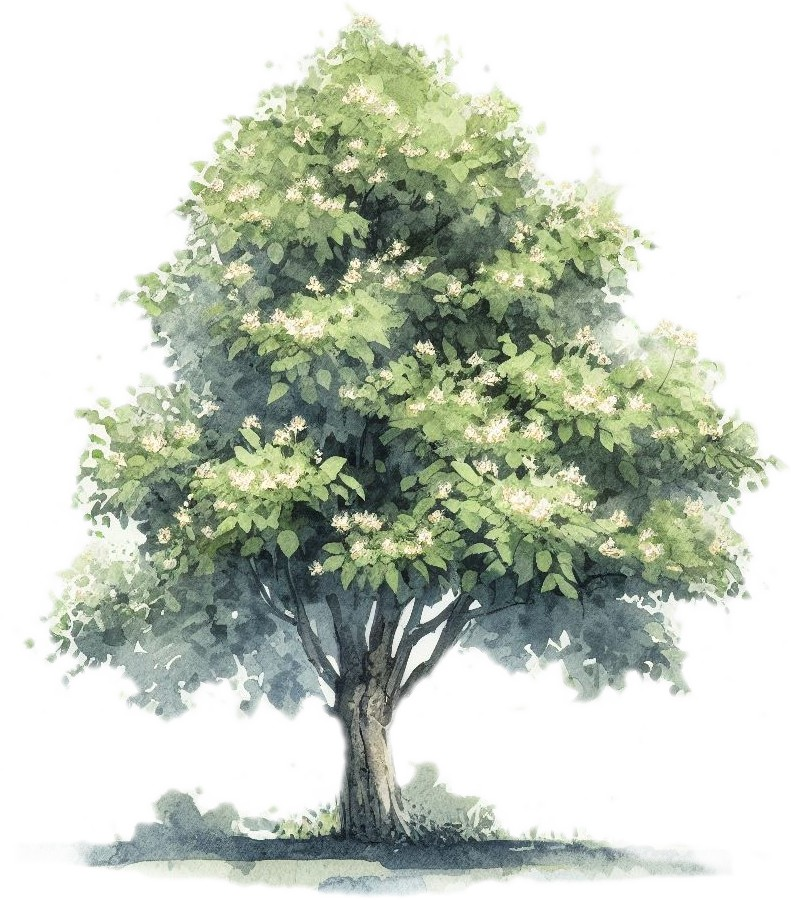
\includegraphics[height=4cm]{images/tree-guide/linden-tree} \\
\hspace{-0.5cm}		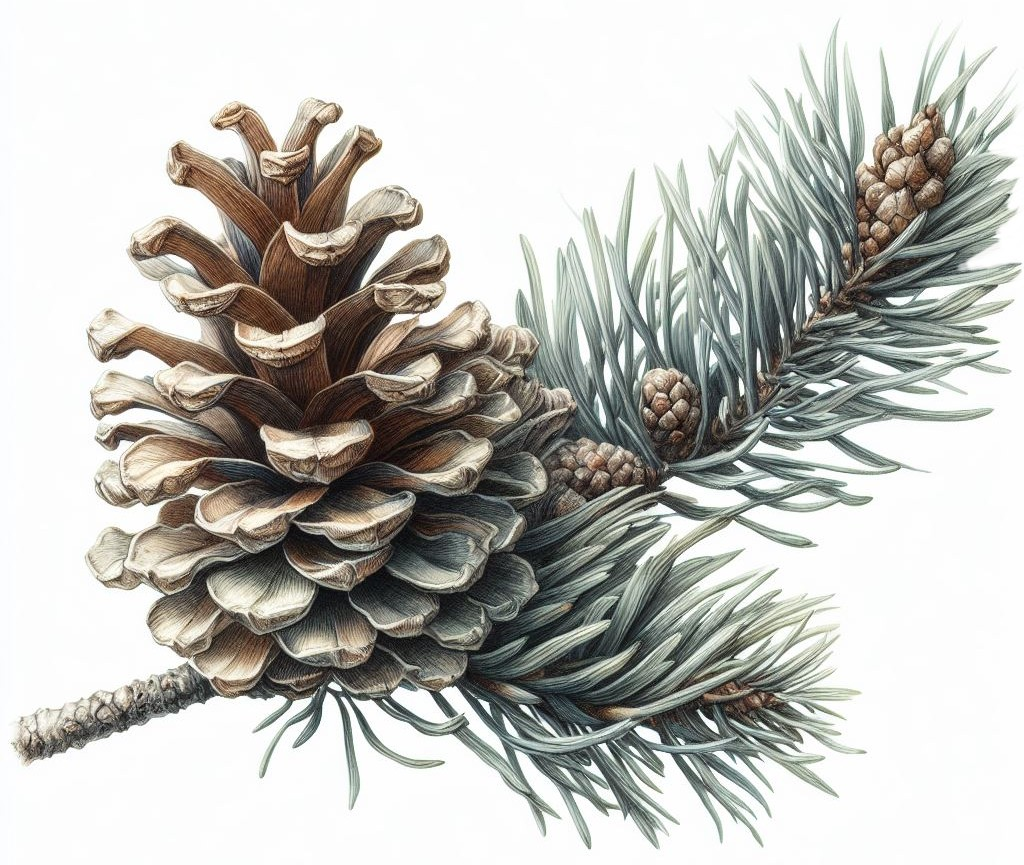
\includegraphics[height=3.5cm]{images/tree-guide/pine-cone-needle} & 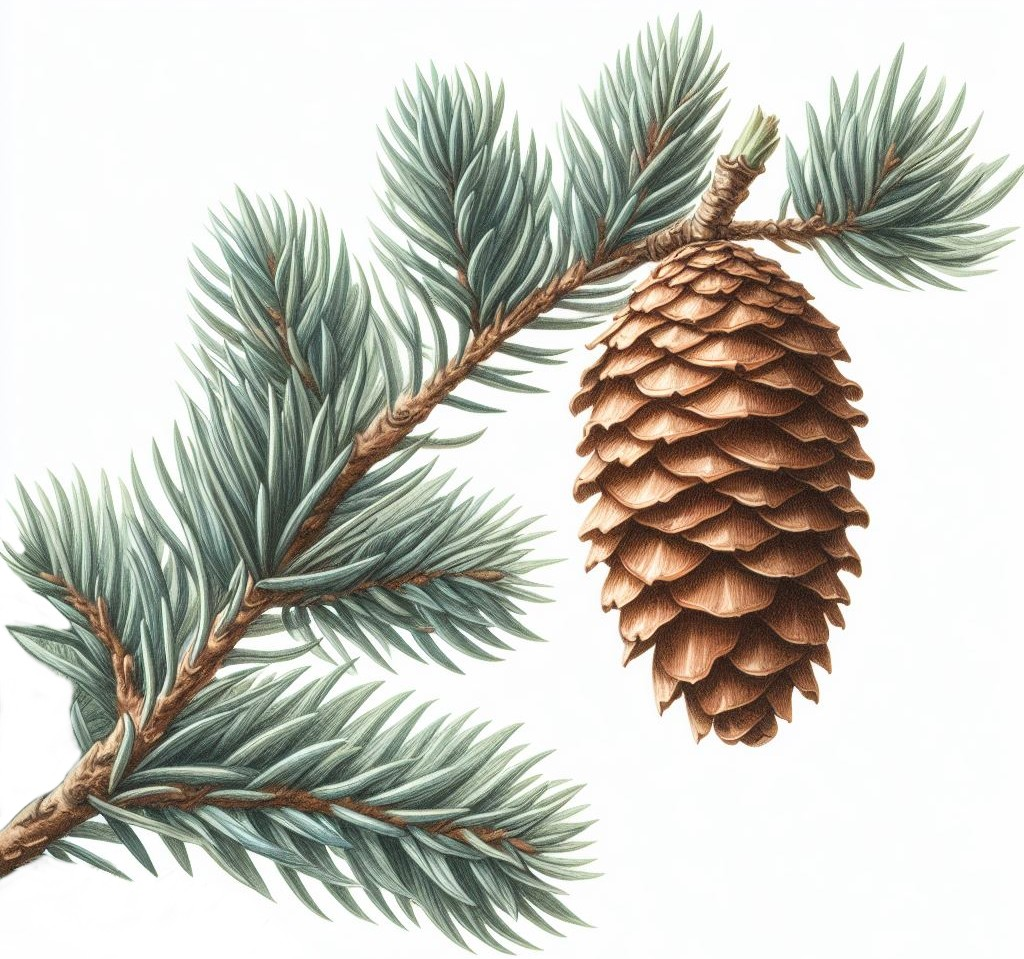
\includegraphics[height=4cm]{images/tree-guide/spruce-cone} &
		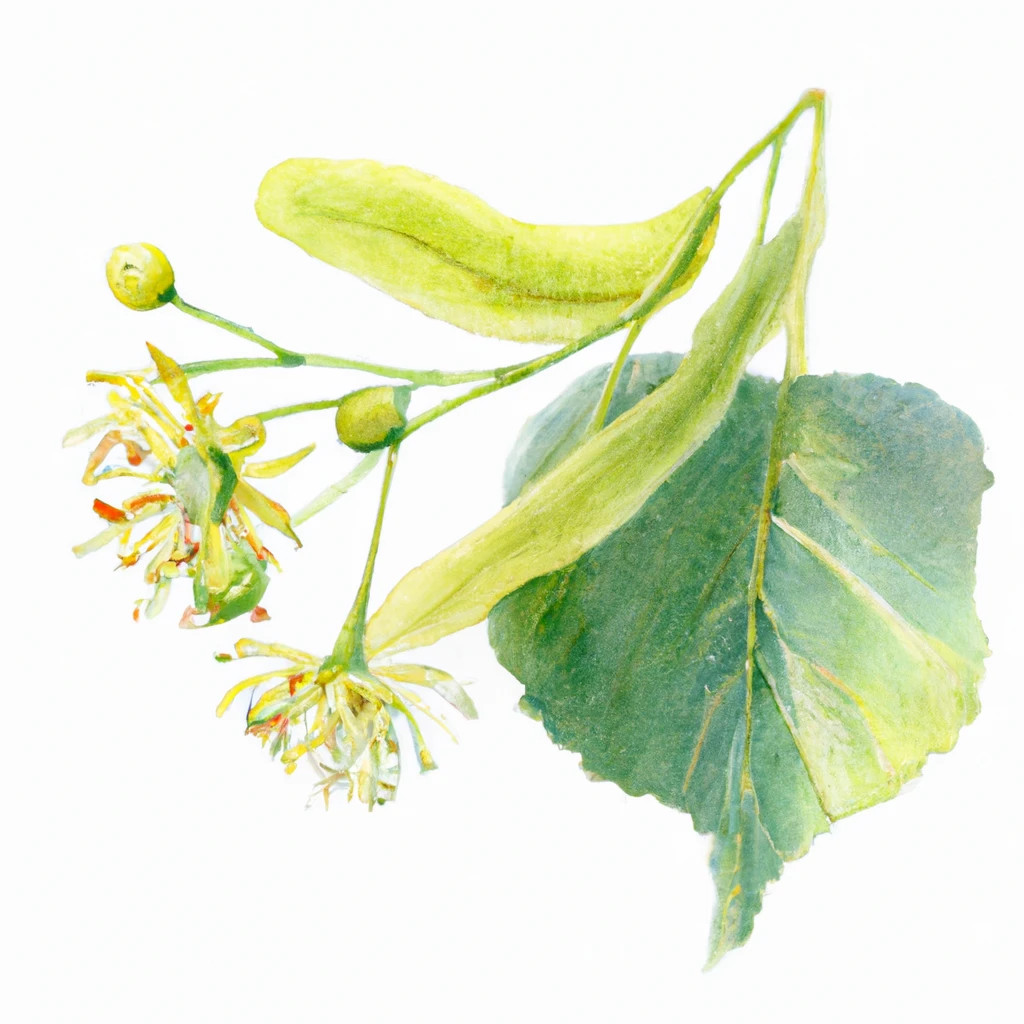
\includegraphics[height=4cm]{images/tree-guide/linden-leaf-blossom} \\
		Сосна, шишка       &  Ель, шишка   &     Липа  \\    
		Pin, con       &  Brad, con    &     Tei  \\    
		Pine, cone        &  Spruce, cone	  & Linden \\    
		die Kiefer, der Zapfen &  die Fichte, der Zapfen    &     die Linden\\    
	\end{tabular}
\end{table}




% PICS to add
%- leaf shapes
%- rhino
%- elephant
%- antilope
%- wildebeast



%She walked along the river Schari all the way up to lake Chad.


%Swallows from Moldova and Romania feel like at home here (because of the similarity of flags).
% https://ru.wikipedia.org/wiki/%D0%A0%D0%BE%D0%B5%D0%B2%D0%BE%D0%B9_%D0%B8%D0%BD%D1%82%D0%B5%D0%BB%D0%BB%D0%B5%D0%BA%D1%82






%- Как же я сам не догадался смотреть на следы? Подумал секретарь. 
%- наверное ты не привык к следам, ведь во время полёта ты следов не оставляешь 
%- да, именно так! Ты смышленнная, прошла мой тест :-) 


%Gestalt drawing of zebra and secretary bird, visible only as black stripes and feathers.








%\newpage
%\section*{Верблюд, который не заблудился}

%\newpage
%\section*{Ласточка, которая не заблудилась}


%\newpage
%\section*{Медведь, который не заблудился}



% this is the back-cover of the book, we ensure there's
% a blank page before it, this makes it easier to produce booklets
\cleartorecto 
\thispagestyle{empty}  % to not have a page# here


\section*{Другие книги нашего издательства}
% \vspace{2cm}

\begin{table}[h]
\begin{tabular}{ccc}

\includegraphics[height=4cm]{images/cava-bien} & 
\includegraphics[height=4cm]{images/suslik} & 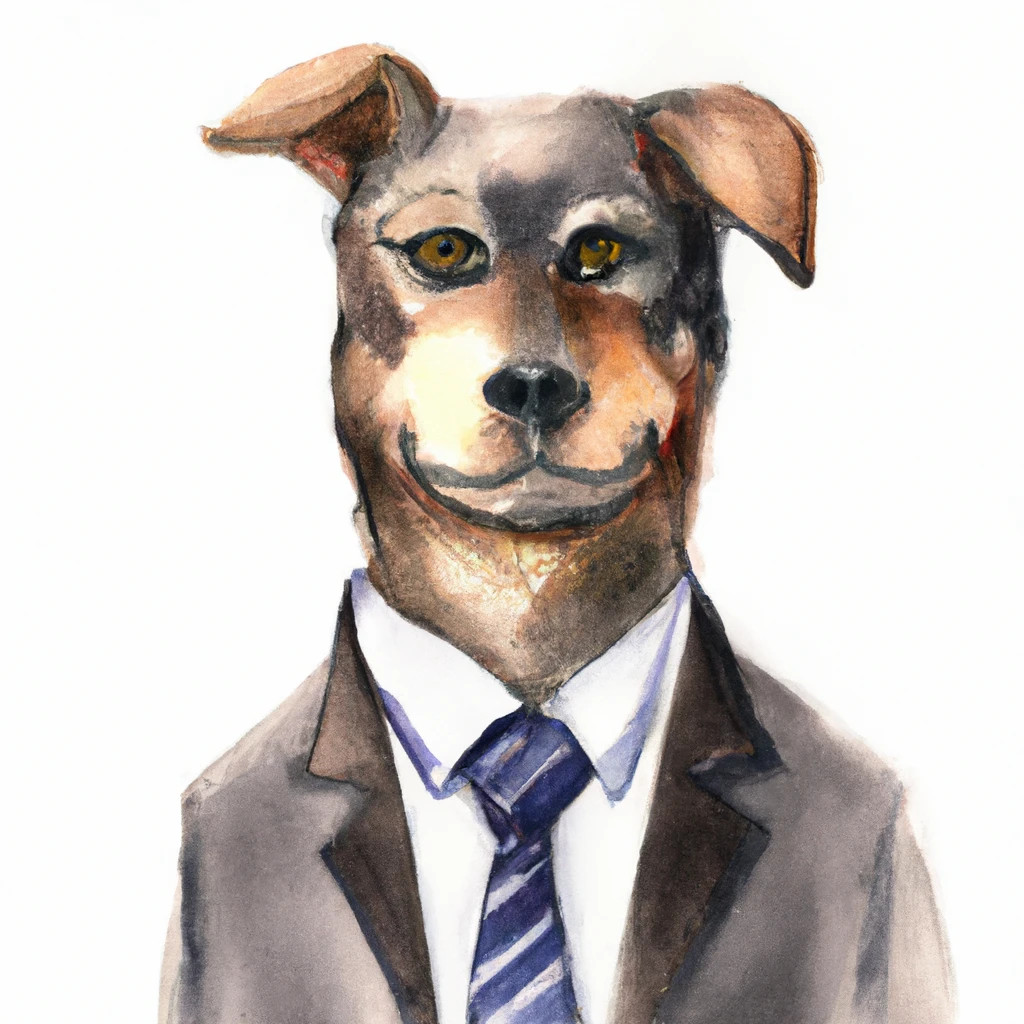
\includegraphics[height=4cm]{images/sobachevich}             \\
 Сова Бьен и Тихо-  &  Сусленский суслик        &   Собакевич и            \\
 Океанский Северо-Запад           &          &    велосипедисты          \\
% Один день из жизни господина Собакевича            
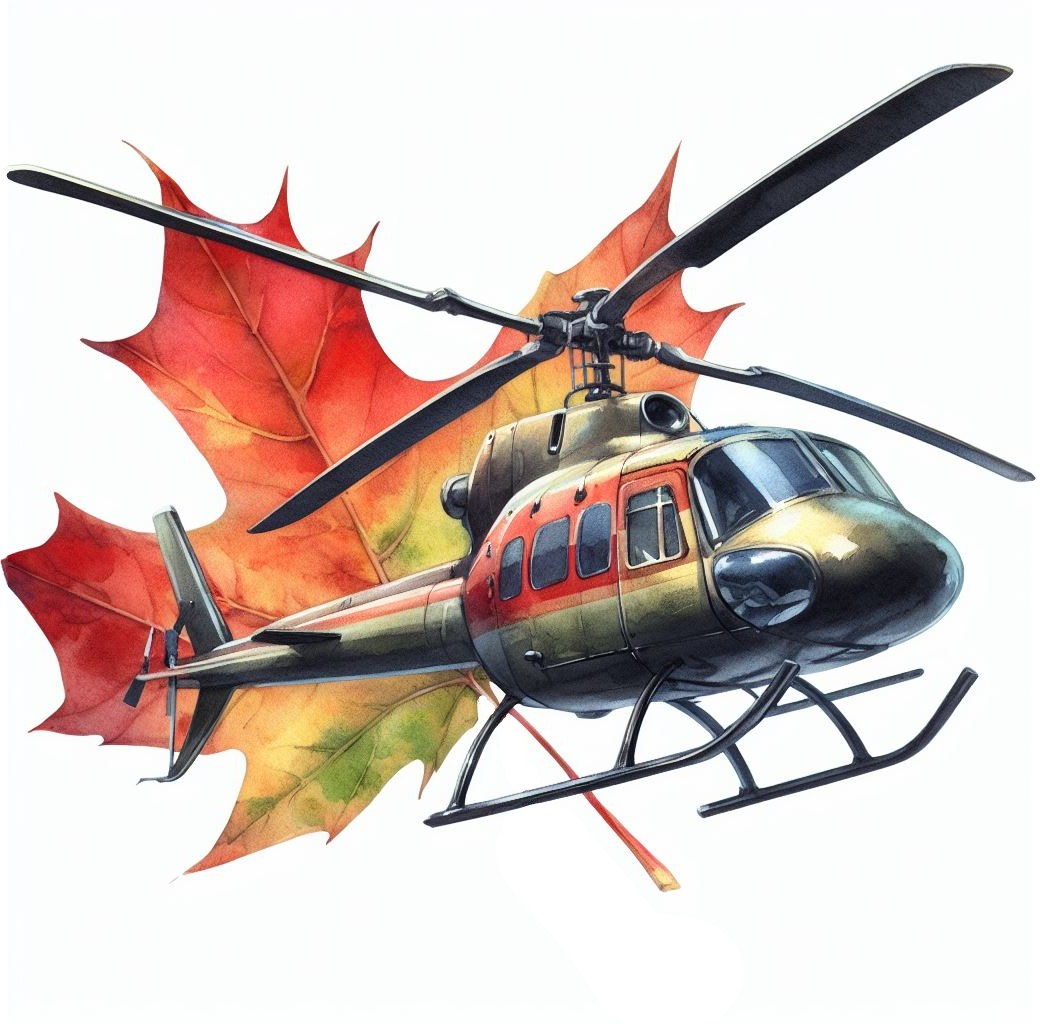
\includegraphics[height=4cm]{images/maple-chopper} & 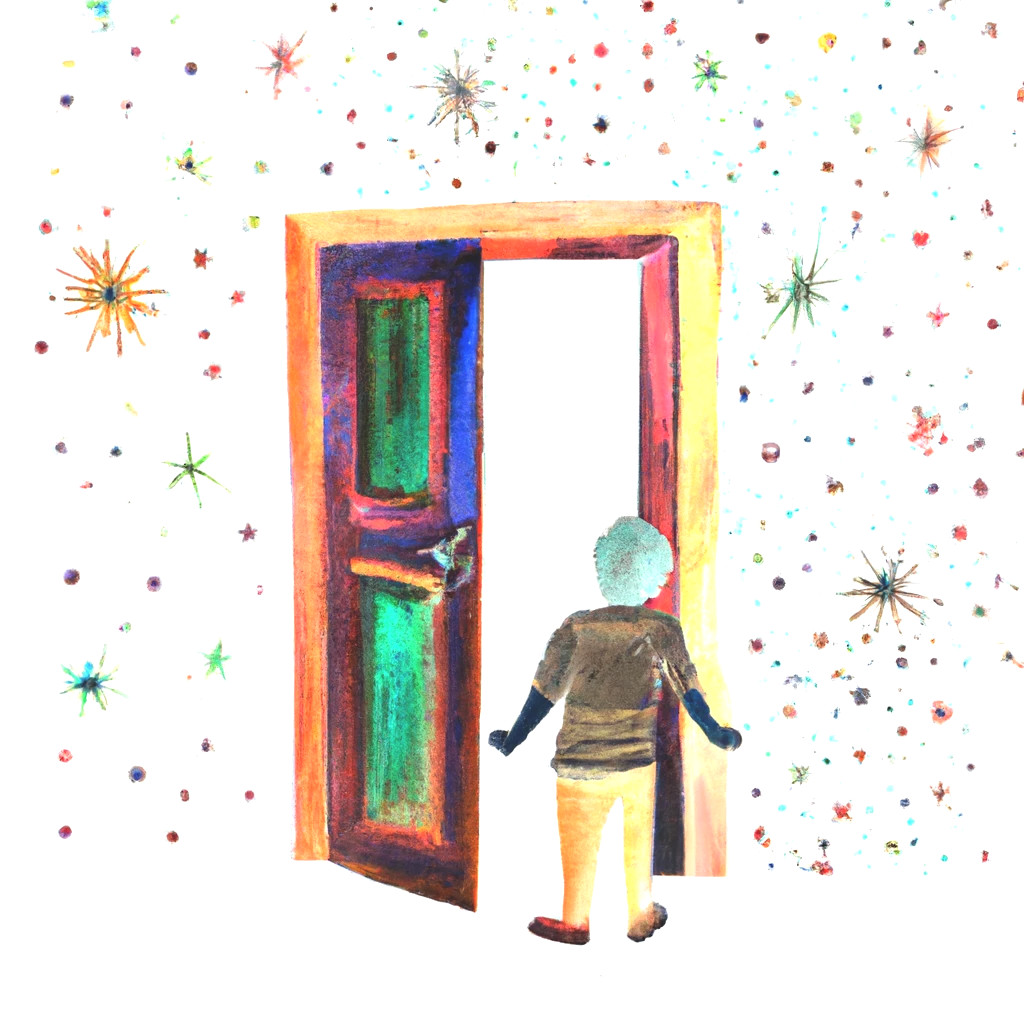
\includegraphics[height=4cm]{images/cosmoroom.jpeg} & 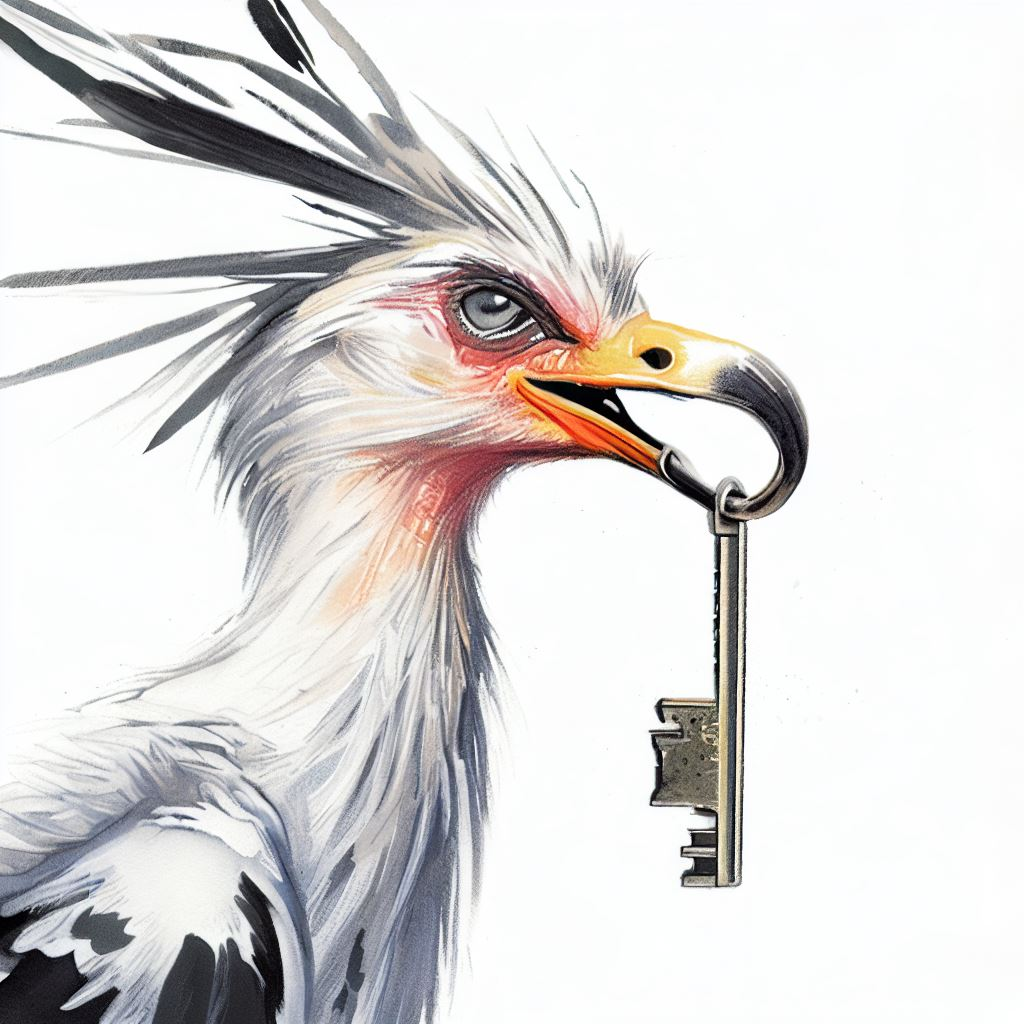
\includegraphics[height=4cm]{images/secretary-key-2}             \\
 Клён и вертолётик       &  Дверь в космос    &     Секретный ключ  \\    
        &      &  секретаря    \\
\end{tabular}
\end{table}

\subsection{Автор и обратная связь}
\hspace{-1cm}
\noindent
\begin{tabular}{p{12cm}p{2cm}}
\footnotesize{Это истории из частично-восстановленного архива, найденного среди развалин архаического вычислительного центра, на дне озера $0x\Sigma \alpha \phi^4_5\bigoplus$. Исходя из метаданных, они были написаны в первой половине XXI века Ручной эпохи Досингулярной эры. Предполагаемое имя автора Papa de la M{\"u}nchen, или Папа де ла Мюнхен, или Папа Мюнхенксий (возможно искажение транслитерации). % Среди блоков данных был найден и фрагмент который не поддавался текстовой интерпретации, мы прилагаем его в виде двухмерной монохромной матрицы. Остальные двухмерные матрицы в сборнике были сгенерированны нами, исходя из контекста.
О неточностях и ошибках сообщайте в Департамент Интерпретаций: alex\faIcon{cat}railean.net.} & \hspace{-5mm}\raisebox{-2.2cm}{ 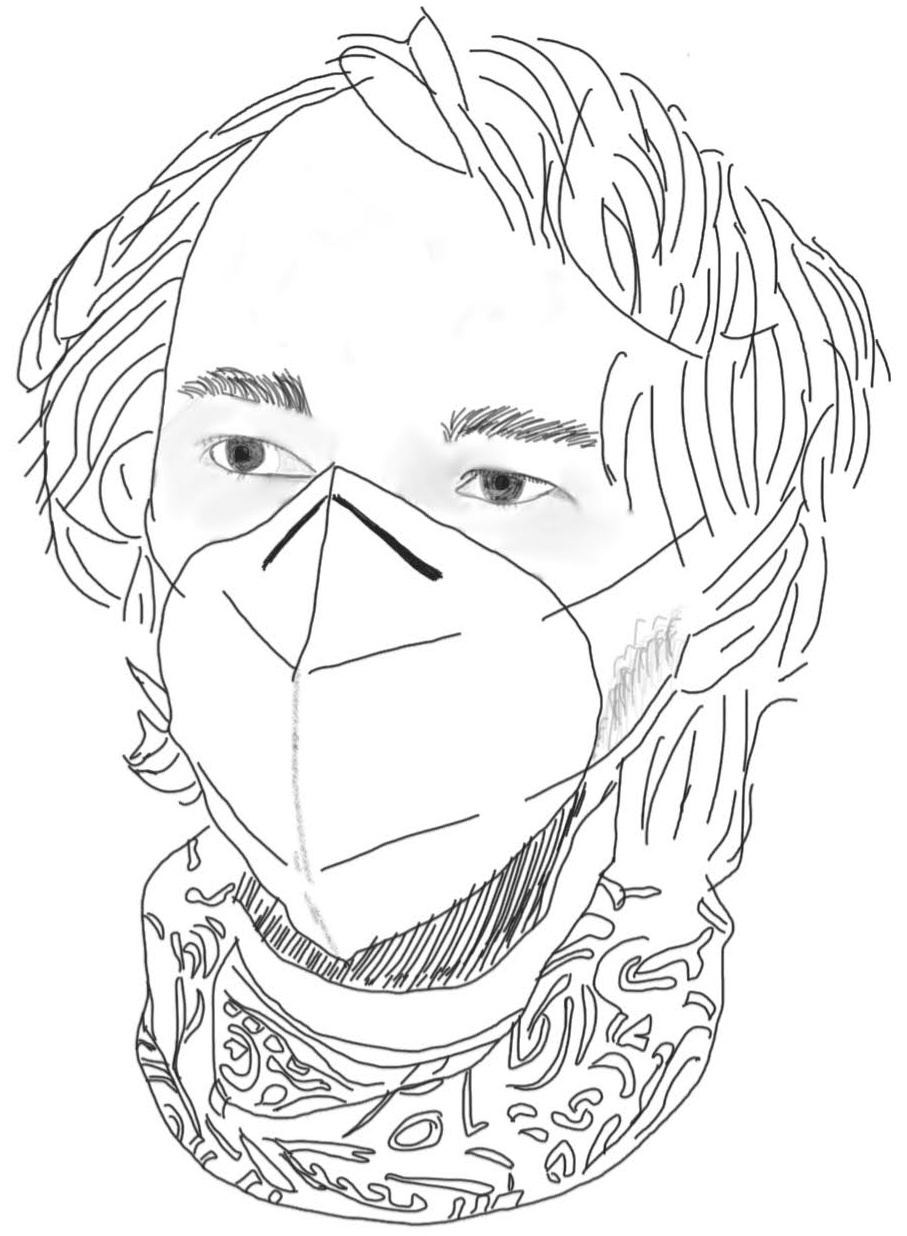
\includegraphics[height=2.5cm]{images/maskavatar-trimmed.jpg}} \\


\includegraphics[height=1.3cm]{images/payments/qr-btc.pdf} \hspace{0.5cm} 
\includegraphics[height=1.3cm]{images/payments/qr-eth.pdf} \hspace{0.5cm} \href{https://paypal.me/ralienpp}{
\includegraphics[height=1.3cm]{images/payments/qr-paypal.pdf}} \hspace{5cm} \href{https://creativecommons.org/licenses/by-sa/4.0/}{\includegraphics[height=0.3cm]{images/cc-by-sa.eps}}&
\end{tabular}

\end{document}


